\documentclass{hcmut-report}
\usepackage{tabularx}
\usepackage{longtable}
\usepackage{multirow}
\usepackage{array}
\usepackage{float}
\usepackage{listings}
\usepackage{xcolor}
\usepackage{etoolbox}
\AtBeginEnvironment{table}{\singlespacing}

% --- Cau hinh chong tran le (Overflow Prevention) & Bang chuan ---
\sloppy
\emergencystretch=3em
\renewcommand{\arraystretch}{1.26}
\setlength{\tabcolsep}{4.5pt}
\newcolumntype{Y}{>{\raggedright\arraybackslash}X}
\newcolumntype{P}[1]{>{\raggedright\arraybackslash}p{#1}}
\newcolumntype{C}[1]{>{\centering\arraybackslash}p{#1}}

% --- Cau hinh hien thi ma nguon gon nhe ---
\definecolor{codebg}{RGB}{248,249,250}
\definecolor{codeframe}{RGB}{180,180,180}
\definecolor{codekw}{RGB}{0,92,197}
\definecolor{codecmt}{RGB}{34,134,58}
\definecolor{codestr}{RGB}{215,58,73}

\lstset{
  backgroundcolor=\color{codebg},
  frame=single,
  rulecolor=\color{codeframe},
  basicstyle=\footnotesize\ttfamily,
  keywordstyle=\color{codekw}\bfseries,
  commentstyle=\color{codecmt}\itshape,
  stringstyle=\color{codestr},
  numbers=left,
  numberstyle=\tiny\color{gray},
  numbersep=5pt,
  xleftmargin=12pt,
  xrightmargin=4pt,
  breaklines=true,
  breakatwhitespace=false,
  showstringspaces=false,
  tabsize=2,
  captionpos=b
}

% --- Thong tin Bia Bao cao (HCMUT - Khoa KH&KT May tinh) ---
\deptname{Faculty of Computer Science and Engineering}
\labname{}
\shortlabname{IoT -- HK261}
\coursename{Internet of Things (IoT) -- Học kỳ 261}
\reporttype{Đặc tả Kỹ thuật \& Kế hoạch Bài tập lớn}
\title{\LARGE\bfseries HỆ THỐNG RADAR KHÔNG CAMERA (WI-FI CSI \& BLE)\\[4pt]\LARGE\bfseries PHÁT HIỆN TÉ NGÃ VÀ XÂM NHẬP TÍCH HỢP AI TẠI BIÊN}
\advisorlabel{Giảng viên hướng dẫn}
\advisor{& TS. Nguyễn Hòa Hưng}
\studentlabel{Nhóm sinh viên}
\stuname{%
  & Lê Ngọc Uy Phong & (MSSV: 2352905) \\
  & Huỳnh Võ Quỳnh Anh & (MSSV: 2452043) \\
  & Trần Thị Bình & (MSSV: 2452157)
}
\reportplace{TP. Hồ Chí Minh}
\reporttime{Tháng 11 năm 2026}

\begin{document}

\coverpage

% =========================================================================
% THONG TIN CHUNG, PHAN CONG NHIEM VU & TU DANH GIA CONG NGHE
% =========================================================================
\section*{Thông tin Nhóm và Sản phẩm Bàn giao}
\addcontentsline{toc}{section}{Thông tin Nhóm và Sản phẩm Bàn giao}

\begin{table}[H]
\centering
\caption{Danh sách thành viên nhóm thực hiện Bài tập lớn IoT (Học kỳ 261)}
\label{tab:group_members}
\small
\begin{tabularx}{\textwidth}{|C{1.0cm}|P{4.8cm}|C{2.4cm}|Y|}
\hline
\textbf{STT} & \textbf{Họ và tên sinh viên} & \textbf{Mã số SV} & \textbf{Thư điện tử học vụ (Email)} \\
\hline
1 & Lê Ngọc Uy Phong & 2352905 & \texttt{phong.le9999@hcmut.edu.vn} \\
\hline
2 & Huỳnh Võ Quỳnh Anh & 2452043 & \texttt{anh.huynhvo02@hcmut.edu.vn} \\
\hline
3 & Trần Thị Bình & 2452157 & \texttt{binh.tranbinh2856@hcmut.edu.vn} \\
\hline
\end{tabularx}
\end{table}

\begin{table}[H]
\centering
\caption{Thông tin các hạng mục bàn giao dự kiến (Submission Information)}
\label{tab:submission_info}
\small
\begin{tabularx}{\textwidth}{|P{4.5cm}|Y|}
\hline
\textbf{Hạng mục bàn giao} & \textbf{Đường dẫn / Thông tin chi tiết} \\
\hline
Tên đề tài tiếng Việt & Hệ thống Radar Không Camera (Wi-Fi CSI \& BLE) Phát hiện Té ngã và Xâm nhập Tích hợp AI tại Biên \\
\hline
Tên đề tài tiếng Anh & Privacy-Preserving Device-Free Indoor Fall \& Intrusion Detection System using Wi-Fi CSI, BLE, and Edge AI \\
\hline
GitHub Repository & \texttt{https://github.com/\allowbreak hcmut-iot-hk261/\allowbreak wifi-csi-fall-detection} \\
\hline
Video Demo (5--10 phút) & \texttt{https://youtu.be/\allowbreak [Cap-nhat-link-video-demo-tuan-16]} \\
\hline
CoreIOT Public Dashboard & \texttt{https://app.coreiot.io/\allowbreak dashboard/\allowbreak [Cap-nhat-UUID-dashboard]} \\
\hline
Hạn nộp cuối cùng & Tuần 16 -- Học kỳ 261 (Năm học 2026--2027) trên hệ thống LMS \\
\hline
\end{tabularx}
\end{table}

\section*{Bảng Phân công Nhiệm vụ Thành viên (Task Assignment Table)}
\addcontentsline{toc}{section}{Bảng Phân công Nhiệm vụ Thành viên}

Bảng \ref{tab:task_assignment} quy định rõ phạm vi công việc, các mã công nghệ phụ trách và tỷ lệ đóng góp của từng thành viên nhằm đảm bảo mỗi sinh viên nắm vững chuyên môn khi bảo vệ vấn đáp và thể hiện rõ lịch sử đóng góp (\texttt{git commit}) trên GitHub.

\begin{table}[H]
\centering
\caption{Phân công nhiệm vụ chi tiết và tỷ lệ đóng góp của 3 thành viên}
\label{tab:task_assignment}
\footnotesize
\begin{tabularx}{\textwidth}{|C{0.7cm}|P{3.0cm}|C{1.6cm}|Y|C{1.1cm}|}
\hline
\textbf{TT} & \textbf{Họ và tên} & \textbf{MSSV} & \textbf{Nhiệm vụ phụ trách chính (Gắn mã công nghệ)} & \textbf{Tỷ lệ} \\
\hline
1 & Lê Ngọc Uy Phong & 2352905 & \textbf{Chuyên gia Phần cứng, Firmware \& Truyền thông Nội bộ:} Thiết kế sơ đồ đấu nối 2 mạch YoloUNO (ESP32-S3); tích hợp cảm biến nhiệt ẩm I2C DHT20 (\textbf{T01}); lập trình phát/thu xung ESP-NOW 100\,Hz và trích xuất ma trận CSI tầng PHY (\textbf{T06}); lập trình bộ quét định danh BLE (\textbf{T03}); xây dựng Embedded Web Server cấu hình ngưỡng nhạy và điều khiển còi/đèn tại chỗ (\textbf{T07}). & 34\% \\
\hline
2 & Huỳnh Võ Quỳnh Anh & 2452043 & \textbf{Chuyên gia AI/TinyML, Xử lý Tín hiệu \& Đo kiểm:} Xây dựng công cụ thu thập dữ liệu CSI qua cổng Serial ra CSV (\textbf{T05}); thiết kế bộ lọc số Hampel/Butterworth; huấn luyện mô hình TinyML 1D-CNN nhúng trên ESP32-S3 (\textbf{T04}); phát triển mô hình 2D-CNN Spectrogram tăng tốc bằng GPU trên PC Gateway (\textbf{T09, N04}); chủ trì kịch bản đo kiểm định lượng 50 lần thử ở cự ly 1--3\,m. & 33\% \\
\hline
3 & Trần Thị Bình & 2452157 & \textbf{Chuyên gia IoT Gateway, Đám mây CoreIOT \& OTA:} Phát triển phần mềm PC Local Gateway bằng Python thu thập telemetry và nhận lệnh RPC 2 chiều (\textbf{T08}); thiết kế giao diện Local UI hiển thị bản đồ nhiệt CSI Heatmap 64 sóng mang (\textbf{T10}); đồng bộ Local Gateway với CoreIOT Gateway (\textbf{T15}); thiết kế CoreIOT Dashboard (\textbf{T11}), kịch bản RuleChain (\textbf{T12}), cảnh báo Telegram/Email (\textbf{T13}) và cập nhật OTA (\textbf{T14}). & 33\% \\
\hline
\multicolumn{4}{|r|}{\textbf{Tổng tỷ lệ đóng góp toàn nhóm}} & \textbf{100\%} \\
\hline
\end{tabularx}
\end{table}

\section*{Bảng Tự Đánh giá Mã Công nghệ (Technology Self-Assessment)}
\addcontentsline{toc}{section}{Bảng Tự Đánh giá Mã Công nghệ}

\begin{table}[H]
\centering
\caption{Bảng A -- Đăng ký và tự đánh giá các thành phần công nghệ cơ bản (Tối đa 8.0 điểm)}
\label{tab:tech_self_assessment}
\footnotesize
\renewcommand{\arraystretch}{1.12}
\begin{tabularx}{\textwidth}{|C{0.9cm}|Y|C{1.0cm}|C{1.2cm}|C{1.9cm}|P{2.7cm}|}
\hline
\textbf{Mã} & \textbf{Thành phần công nghệ (Technology Element)} & \textbf{Điểm} & \textbf{Chọn} & \textbf{Mục đặc tả} & \textbf{Minh chứng} \\
\hline
\multicolumn{6}{|l|}{\textbf{Nhóm 1 -- Cảm biến (Sensors)}} \\
\hline
T01 & Cảm biến giao tiếp I2C (DHT20/SHT30) trên Tasmota / ESP32 & 0.5 & \textbf{Có} & Mục 2.3.1, 3.1 & Ảnh mạch, log I2C \\
\hline
T02 & Cảm biến giao tiếp chuẩn công nghiệp Modbus RS485 & 1.0 & Không & -- & -- \\
\hline
T03 & Thiết bị/cảm biến kết nối qua Bluetooth Low Energy (BLE) & 1.5 & \textbf{Có} & Mục 2.3.1, 3.3 & Log MAC/RSSI BLE \\
\hline
\multicolumn{6}{|l|}{\textbf{Nhóm 2 -- Trí tuệ nhân tạo tại biên (On-device TinyML)}} \\
\hline
T04 & Suy luận thông tin bằng mô hình TinyML chạy trực tiếp trên mạch & 1.0 & \textbf{Có} & Mục 2.3.4, 3.5 & Log suy luận $<18$\,ms \\
\hline
T05 & Bộ công cụ thu thập dữ liệu, huấn luyện và xuất mô hình TinyML & 1.0 & \textbf{Có} & Mục 3.5.1, 3.5.2 & Script CSV, TFLite \\
\hline
\multicolumn{6}{|l|}{\textbf{Nhóm 3 -- Giao tiếp và Giao diện nội bộ (Local Communication \& Interfaces)}} \\
\hline
T06 & Truyền thông không dây giữa các mạch bằng giao thức ESP-NOW & 1.5 & \textbf{Có} & Mục 2.3.2, 3.3 & Gói CSI 100\,Hz \\
\hline
T07 & Web Server nhúng tự lập trình trên thiết bị (hiển thị \& điều khiển) & 1.0 & \textbf{Có} & Mục 3.2.3 & Giao diện HTTP \\
\hline
\multicolumn{6}{|l|}{\textbf{Nhóm 4 -- Trạm Local IoT Gateway (PC / Raspberry Pi)}} \\
\hline
T08 & Local Gateway tổng hợp dữ liệu gửi lên CoreIOT và nhận lệnh chiều về & 1.0 & \textbf{Có} & Mục 2.3.3, 3.4 & Code Python Gateway \\
\hline
T09 & Hàm AI chạy trên Local Gateway phân tích dữ liệu và phát hiện sự kiện & 1.0 & \textbf{Có} & Mục 3.5.3 & Spectrogram CNN \\
\hline
T10 & Giao diện giám sát và điều khiển trực quan tại Local IoT Gateway & 1.0 & \textbf{Có} & Mục 3.4.2 & Giao diện Streamlit \\
\hline
\multicolumn{6}{|l|}{\textbf{Nhóm 5 -- Nền tảng Đám mây CoreIOT (CoreIOT Platform)}} \\
\hline
T11 & Sử dụng Template phát triển ứng dụng, Dashboard giám sát từ xa & 1.0 & \textbf{Có} & Mục 3.6.1 & CoreIOT Dashboard \\
\hline
T12 & Sử dụng RuleChain xây dựng các tính năng xử lý thông minh & 1.0 & \textbf{Có} & Mục 3.6.2 & Sơ đồ nút RuleChain \\
\hline
T13 & Gửi thông báo cảnh báo (Telegram/Email) khi dữ liệu vượt ngưỡng & 0.5 & \textbf{Có} & Mục 3.6.2 & Tin nhắn Telegram \\
\hline
T14 & Cập nhật firmware từ xa qua mạng (OTA) cho thiết bị ESP32-S3 & 2.0 & \textbf{Có} & Mục 3.6.3 & Log OTA v1.0$\rightarrow$v1.1 \\
\hline
T15 & Đồng bộ hóa IoT Gateway trên CoreIOT với Local IoT Gateway & 2.0 & \textbf{Có} & Mục 3.4.1, 3.6.1 & Bản ghi Gateway Sync \\
\hline
\multicolumn{2}{|r|}{\textbf{Tổng điểm công nghệ đăng ký}} & \textbf{14.0} & \multicolumn{3}{l|}{\textbf{Quy đổi tối đa: 8.0 / 8.0 điểm}} \\
\hline
\end{tabularx}
\end{table}

\begin{table}[H]
\centering
\caption{Bảng B -- Đăng ký tính năng nâng cao (Advanced Features -- Tối đa 1.0 điểm thưởng)}
\label{tab:adv_self_assessment}
\footnotesize
\renewcommand{\arraystretch}{1.15}
\begin{tabularx}{\textwidth}{|C{0.9cm}|Y|C{1.0cm}|C{1.2cm}|C{1.9cm}|P{2.7cm}|}
\hline
\textbf{Mã} & \textbf{Tính năng nâng cao (Advanced Feature)} & \textbf{Điểm} & \textbf{Chọn} & \textbf{Mục đặc tả} & \textbf{Minh chứng} \\
\hline
N01 & Trợ lý ảo tích hợp mô hình ngôn ngữ lớn (Virtual Assistant -- LLM) & 1.0 & Dự phòng & Mục 3.7 & Chatbot hỏi đáp \\
\hline
N02 & Giao tiếp và điều khiển bằng giọng nói (Voice -- Audio) & 1.0 & Không & -- & -- \\
\hline
N03 & Hiển thị màn hình đồ họa sử dụng thư viện LVGL & 1.0 & Không & -- & -- \\
\hline
N04 & Tăng tốc mô hình AI chạy trên GPU của thiết bị / Gateway & 1.0 & \textbf{Có} & Mục 3.5.3, 3.7 & ONNX Runtime CUDA \\
\hline
N05 & Ứng dụng di động tự thiết kế (Custom-designed Mobile App) & 1.0 & Không & -- & -- \\
\hline
N06 & Dashboard tự thiết kế có khả năng phát hiện và ghi nhận sự kiện & 1.0 & \textbf{Có} & Mục 3.4.2, 3.7 & Nhật ký + Heatmap \\
\hline
N07 & Tự triển khai máy chủ ThingsBoard cục bộ (Self-deployed ThingsBoard) & 1.0 & Không & -- & -- \\
\hline
\multicolumn{2}{|r|}{\textbf{Tổng điểm nâng cao đăng ký}} & \textbf{2.0} & \multicolumn{3}{l|}{\textbf{Quy đổi tối đa: 1.0 / 1.0 điểm}} \\
\hline
\end{tabularx}
\end{table}

\section*{Danh mục Từ viết tắt (List of Abbreviations)}
\addcontentsline{toc}{section}{Danh mục Từ viết tắt}

\begin{table}[H]
\centering
\small
\begin{tabularx}{\textwidth}{|P{2.2cm}|P{5.5cm}|Y|}
\hline
\textbf{Từ viết tắt} & \textbf{Thuật ngữ tiếng Anh} & \textbf{Giải nghĩa tiếng Việt} \\
\hline
BLE & Bluetooth Low Energy & Chuẩn truyền thông không dây Bluetooth năng lượng thấp \\
\hline
CNN & Convolutional Neural Network & Mạng nơ-ron tích chập (1D-CNN tại biên và 2D-CNN trên Gateway) \\
\hline
CSI & Channel State Information & Thông tin trạng thái kênh truyền sóng vô tuyến Wi-Fi ở tầng PHY \\
\hline
ESP-NOW & Espressif Connectionless Wi-Fi & Giao thức truyền thông không dây ngang hàng độ trễ thấp của Espressif \\
\hline
HAR & Human Activity Recognition & Nhận diện hành vi và hoạt động của con người \\
\hline
I2C & Inter-Integrated Circuit & Chuẩn giao tiếp nối tiếp đồng bộ hai dây (SDA và SCL) \\
\hline
MQTT & Message Queuing Telemetry Transport & Giao thức truyền thông điệp nhẹ theo mô hình Publish/Subscribe \\
\hline
OFDM & Orthogonal Frequency-Division Multiplexing & Ghép kênh phân chia theo tần số trực giao (64 sóng mang phụ) \\
\hline
OTA & Over-The-Air Firmware Update & Cơ chế cập nhật phần mềm nhúng từ xa qua mạng không dây \\
\hline
RSSI & Received Signal Strength Indicator & Chỉ số cường độ tín hiệu thu được (đơn vị dBm) \\
\hline
STFT & Short-Time Fourier Transform & Biến đổi Fourier thời gian ngắn dùng để tạo ảnh phổ Spectrogram \\
\hline
TinyML & Tiny Machine Learning & Học máy siêu nhỏ gọn chạy trực tiếp trên vi điều khiển (ESP32-S3) \\
\hline
\end{tabularx}
\end{table}

\newpage
\tableofcontents
\newpage

% =========================================================================
% CHUONG 1: GIOI THIEU (INTRODUCTION)
% =========================================================================
\section[Giới thiệu]{Giới thiệu (Introduction)}

\subsection[Đặt vấn đề]{Đặt vấn đề (Problem Statement)}
Theo báo cáo thống kê y tế toàn cầu của Tổ chức Y tế Thế giới (WHO), té ngã là nguyên nhân đứng thứ hai gây tử vong do chấn thương không chủ ý trên toàn thế giới, đặc biệt nguy hiểm đối với người cao tuổi sống độc thân hoặc bệnh nhân đang phục hồi chức năng \cite{wang2017wifall}. Tại Việt Nam cũng như nhiều quốc gia đang già hóa dân số, phần lớn các tai nạn té ngã nghiêm trọng xảy ra tại các khu vực nhạy cảm trong nhà như phòng tắm, phòng ngủ hoặc hành lang vào ban đêm. Nếu nạn nhân nằm bất động sau cú ngã mà không được phát hiện và cấp cứu trong ``khung giờ vàng'' (30--60 phút đầu tiên), nguy cơ biến chứng tim mạch, hạ thân nhiệt hoặc tử vong sẽ tăng gấp nhiều lần \cite{palipana2018falldefi}.

Bên cạnh bài toán giám sát an toàn sức khỏe cho người già, nhu cầu bảo vệ an ninh nội thất (phát hiện kẻ gian đột nhập vào ban đêm hoặc khi vắng nhà) cũng đòi hỏi một hệ thống giám sát hoạt động liên tục 24/7. Tuy nhiên, các phương pháp tiếp cận truyền thống hiện nay đang vấp phải ba rào cản lớn:
\begin{enumerate}
  \item \textbf{Xâm phạm quyền riêng tư và điểm mù thị giác (Camera giám sát):} Các hệ thống camera AI (Computer Vision) có độ chính xác cao nhưng hoàn toàn không thể lắp đặt trong phòng tắm hoặc phòng ngủ vì lý do riêng tư cá nhân. Hơn nữa, camera bị vô hiệu hóa trong điều kiện tắt đèn tối hoàn toàn, bị khuất tầm nhìn bởi rèm cửa, bàn ghế hoặc vách ngăn mỏng.
  \item \textbf{Sự bất tiện của thiết bị đeo (Wearable IMU Sensors):} Các vòng tay hoặc đồng hồ thông minh tích hợp cảm biến gia tốc (IMU) đòi hỏi người cao tuổi phải đeo trên người 24/24 và sạc pin thường xuyên. Thực tế cho thấy người già rất dễ quên đeo thiết bị, hoặc tháo thiết bị ra đúng lúc đi tắm --- thời điểm dễ xảy ra trượt ngã nhất \cite{halperin2011tool}.
  \item \textbf{Độ nhạy kém của cảm biến hồng ngoại thụ động (PIR):} Cảm biến PIR truyền thống chỉ phát hiện được chuyển động nhiệt thô, không thể phân biệt giữa người đang đi bộ bình thường với người vừa bị té ngã, và hoàn toàn mất tác dụng khi đối tượng nằm bất động sau khi ngã.
\end{enumerate}

Để giải quyết triệt để cả ba hạn chế trên mà không cần đầu tư các cảm biến radar mmWave đắt tiền, đề tài đề xuất xây dựng \textbf{``Hệ thống Radar Không Camera (Wi-Fi CSI \& BLE) Phát hiện Té ngã và Xâm nhập Tích hợp AI tại Biên''} dựa trên nền tảng mạch phát triển \textbf{YoloUNO (ESP32-S3)} và máy chủ đám mây \textbf{CoreIOT}. Hệ thống tận dụng chính sự biến dạng biên độ và pha của 64 sóng mang phụ (subcarriers) trong tín hiệu Wi-Fi \textbf{CSI (Channel State Information)} truyền qua giao thức \textbf{ESP-NOW} giữa hai mạch ESP32-S3 để ``cảm nhận'' chuyển động cơ thể người xuyên qua bóng tối và vật cản mỏng, kết hợp quét tín hiệu định danh \textbf{Bluetooth Low Energy (BLE)} nhằm phân biệt thông minh giữa kịch bản \textit{cấp cứu người nhà bị té ngã} và kịch bản \textit{báo động kẻ lạ đột nhập}.

\subsection[Khảo sát các giải pháp liên quan]{Khảo sát các giải pháp liên quan (Related Solutions)}
Trong những năm gần đây, công nghệ cảm biến không thiết bị đeo (Device-Free Wireless Sensing) sử dụng thông tin trạng thái kênh truyền Wi-Fi (CSI) đã thu hút sự quan tâm lớn từ cộng đồng nghiên cứu học thuật \cite{ma2019survey}. Bảng \ref{tab:related_work} tổng hợp và so sánh các công trình tiêu biểu cũng như các giải pháp thương mại hiện có với hệ thống đề xuất của nhóm.

\begin{table}[H]
\centering
\caption{So sánh các giải pháp phát hiện té ngã và giám sát trong nhà hiện có với hệ thống đề xuất}
\label{tab:related_work}
\footnotesize
\begin{tabularx}{\textwidth}{|P{2.9cm}|P{3.2cm}|Y|Y|}
\hline
\textbf{Giải pháp} & \textbf{Công nghệ cốt lõi} & \textbf{Ưu điểm chính} & \textbf{Hạn chế cần khắc phục} \\
\hline
Vòng đeo tay IMU (Apple Watch / Mi Band) & Gia tốc kế 3 trục + Con quay hồi chuyển (I2C/SPI) & Nhận diện cú va chạm trực tiếp tốt, cảnh báo nhanh khi đang đeo. & Người già hay quên đeo hoặc tháo ra khi đi tắm; phải sạc pin liên tục. \\
\hline
Camera AI Giám sát (YOLO / MediaPipe) & Xử lý ảnh qua mạng CNN trên camera IP & Trực quan, nhận diện tư thế ngã chính xác khi đủ ánh sáng. & Xâm phạm nghiêm trọng quyền riêng tư (phòng tắm/phòng ngủ); bị che khuất bởi vật cản. \\
\hline
Hệ thống WiFall \cite{wang2017wifall} \& FallDeFi \cite{palipana2018falldefi} & Intel 5300 NIC thu Wi-Fi CSI + Máy tính chạy SVM / Random Forest & Không cần đeo thiết bị, bảo mật riêng tư 100\%, hoạt động xuyên bóng tối. & Đòi hỏi card mạng máy tính chuyên dụng cồng kềnh, không có suy luận AI tại biên (TinyML) hay quản trị đám mây IoT. \\
\hline
ESP32-CSI-Tool \cite{hernandez2020lightweight} \& Espressif \texttt{esp-csi} \cite{espressif_csi} & Thu thập CSI trên vi điều khiển ESP32 chi phí thấp & Gọn nhẹ, không cần card mạng Intel 5300, dễ triển khai nhiều node. & Mới dừng ở mức công cụ thu thập dữ liệu thô; thiếu cơ chế định danh BLE và nền tảng cảnh báo IoT hoàn chỉnh. \\
\hline
\textbf{Hệ thống Đề xuất của Nhóm (BTL HK261)} & \textbf{2 Node YoloUNO (ESP32-S3) + ESP-NOW CSI + BLE + TinyML + GPU Gateway + CoreIOT} & \textbf{Bảo vệ 100\% riêng tư; không cần đeo cảm biến; AI 2 tầng (TinyML + GPU Spectrogram); kết hợp BLE phân biệt Người nhà / Kẻ trộm; đồng bộ CoreIOT \& OTA.} & Phạm vi tối ưu trong 1 phòng kín ($3\,\text{m} \times 4\,\text{m}$); cần cố định vị trí 2 node Tx và Rx. \\
\hline
\end{tabularx}
\end{table}

\subsection[Mục tiêu của Đề tài]{Mục tiêu của Đề tài (Project Objectives)}
Đề tài đặt ra mục tiêu tổng quát là thiết kế, chế tạo và kiểm chứng thực nghiệm một hệ thống IoT hoàn chỉnh theo kiến trúc kết hợp \textbf{Edge AI -- Local IoT Gateway -- CoreIOT Cloud}. Các mục tiêu kỹ thuật định lượng (sẽ được đo kiểm và đối chiếu tại Chương 4) bao gồm:
\begin{enumerate}
  \item \textbf{Tốc độ lấy mẫu sóng vô tuyến ổn định:} Duy trì luồng phát/thu gói tin ESP-NOW giữa Node 1 (Tx) và Node 2 (Rx) ở tần số lấy mẫu $f_s = 50\text{--}100\,\text{Hz}$ trên 64 sóng mang phụ OFDM với tỷ lệ mất gói (packet loss rate) dưới $2\%$ ở khoảng cách $1\text{--}4\,\text{m}$.
  \item \textbf{Độ chính xác nhận diện hành vi và té ngã:} Mô hình TinyML (1D-CNN lượng tử hóa INT8) chạy trên ESP32-S3 đạt độ chính xác phân loại 4 trạng thái (\texttt{Empty}, \texttt{Stationary}, \texttt{Walking}, \texttt{Fall}) trên $88\%$ với thời gian suy luận tại biên dưới $25\,\text{ms}$; mô hình xác thực chéo 2D-CNN Spectrogram trên GPU của PC Local Gateway đạt điểm F1-score trên $92\%$.
  \item \textbf{Độ trễ cảnh báo đầu-cuối (End-to-End Alert Latency):} Tổng thời gian từ lúc xảy ra sự kiện té ngã thực tế đến khi còi báo động tại chỗ kêu là dưới $0.8\,\text{giây}$, và đến khi tin nhắn cảnh báo khẩn cấp xuất hiện trên Telegram / CoreIOT Dashboard là dưới $2.0\,\text{giây}$.
  \item \textbf{Khả năng quản trị và cập nhật từ xa:} Đồng bộ hóa 100\% trạng thái đa thiết bị giữa Local IoT Gateway và CoreIOT Gateway (\textbf{T15}), đồng thời thực hiện thành công quy trình cập nhật firmware từ xa qua mạng (\textbf{OTA -- T14}) trong thời gian dưới $60\,\text{giây}$.
\end{enumerate}

\subsection[Danh sách Tính năng Hệ thống Đề xuất]{Danh sách Tính năng Hệ thống Đề xuất (Proposed System Features)}
Bảng \ref{tab:system_features} định nghĩa cụ thể 10 tính năng cốt lõi của hệ thống (ký hiệu từ \textbf{F01} đến \textbf{F10}), thiết bị thực thi tương ứng và mức độ ưu tiên.

\begin{table}[H]
\centering
\caption{Danh sách các tính năng cụ thể và có thể kiểm chứng của hệ thống (F01--F10)}
\label{tab:system_features}
\footnotesize
\renewcommand{\arraystretch}{1.12}
\begin{tabularx}{\textwidth}{|C{0.8cm}|Y|P{3.4cm}|C{1.5cm}|}
\hline
\textbf{Mã} & \textbf{Mô tả chi tiết tính năng (Specific \& Verifiable Description)} & \textbf{Thiết bị thực thi} & \textbf{Ưu tiên} \\
\hline
F01 & Phát liên tục các khung tin không dây ESP-NOW ở tần số $100\,\text{Hz}$ từ Node 1 sang Node 2 và trích xuất ma trận biên độ/pha của 64 sóng mang Wi-Fi CSI ở tầng vật lý (PHY). & Node 1 (Tx) \& Node 2 (Rx) & Bắt buộc \\
\hline
F02 & Đọc nhiệt độ ($^\circ\text{C}$) và độ ẩm tương đối ($\%\text{RH}$) mỗi 5 giây qua cảm biến I2C DHT20, đóng gói kèm khung ESP-NOW để hiệu chuẩn đường nền (baseline) của biên độ sóng CSI. & Node 1 (YoloUNO \#1 + DHT20) & Bắt buộc \\
\hline
F03 & Quét định kỳ mỗi 1 giây các gói quảng bá Bluetooth Low Energy (BLE Advertising) xung quanh phòng, trích xuất địa chỉ MAC và chỉ số RSSI để xác thực sự hiện diện của chủ nhà. & Node 2 (YoloUNO \#2) \& BLE Tag & Bắt buộc \\
\hline
F04 & Thu thập dữ liệu CSI qua cổng Serial thành tập tin CSV, tiền xử lý bằng bộ lọc Hampel/Butterworth và chạy mô hình TinyML 1D-CNN trực tiếp trên ESP32-S3 để phân loại 4 trạng thái: Phòng trống (\texttt{Empty}), Đứng yên (\texttt{Stationary}), Đi lại (\texttt{Walking}) và Té ngã (\texttt{Fall}). & Node 2 (ESP32-S3) \& PC Tooling & Bắt buộc \\
\hline
F05 & Cung cấp giao diện Web Server nhúng trực tiếp trên Node 2 (truy cập qua trình duyệt nội bộ) cho phép xem trạng thái tức thời, chỉnh ngưỡng độ nhạy phát hiện ngã và kiểm thử còi/đèn. & Node 2 (Embedded HTTP Server) & Bắt buộc \\
\hline
F06 & Kích hoạt tức thời còi báo động Buzzer ($2.7\,\text{kHz}$) và dải đèn LED RGB WS2812B nháy đỏ khi phát hiện té ngã, kèm nút nhấn vật lý cho phép người dùng hủy báo động giả hoặc bấm giữ 3 giây để phát tín hiệu SOS khẩn cấp. & Node 2 (Buzzer, NeoPixel, Nút SOS) & Bắt buộc \\
\hline
F07 & Vận hành dịch vụ Local IoT Gateway trên PC thu thập luồng dữ liệu tốc độ cao từ Node 2 qua USB-CDC/MQTT, đồng bộ hóa thiết bị với CoreIOT Gateway và phân phối lệnh điều khiển RPC chiều về xuống các node. & PC Local Gateway \& CoreIOT & Bắt buộc \\
\hline
F08 & Biến đổi chuỗi CSI sang ảnh phổ thời gian--tần số (STFT Spectrogram), chạy mô hình 2D-CNN tăng tốc bằng GPU trên PC Gateway để xác thực chéo sự kiện té ngã và hiển thị bản đồ nhiệt 64 kênh theo thời gian thực trên giao diện Local UI. & PC Local Gateway (GPU + Streamlit) & Bắt buộc \\
\hline
F09 & Thực thi kịch bản tự động hóa trên CoreIOT RuleChain: (1) Nếu \texttt{state == FALL} thì phát lệnh cấp cứu y tế; (2) Nếu \texttt{state == WALKING} nhưng \texttt{ble\_authorized == false} thì phát cảnh báo xâm nhập trái phép qua Telegram Bot và Email. & CoreIOT Server (RuleChain) & Bắt buộc \\
\hline
F10 & Giám sát và điều khiển toàn bộ hệ thống từ xa qua CoreIOT Dashboard (sử dụng Device Profile \& Template) và hỗ trợ nâng cấp firmware từ xa qua mạng (OTA) cho các mạch YoloUNO. & CoreIOT Server \& Node 1, Node 2 & Mở rộng \\
\hline
\end{tabularx}
\end{table}

\subsection[Phạm vi và Giới hạn của Đề tài]{Phạm vi và Giới hạn của Đề tài (Scope and Limitations)}
\begin{itemize}
  \item \textbf{Phạm vi triển khai:} Hệ thống được thiết kế và thử nghiệm trong không gian một phòng kín tiêu chuẩn có diện tích từ $9\,\text{m}^2$ đến $16\,\text{m}^2$ (khoảng cách trực diện giữa Node 1 và Node 2 từ $1.5\,\text{m}$ đến $3.5\,\text{m}$), tập trung vào bài toán giám sát một người cao tuổi sinh hoạt trong phòng hoặc phát hiện một đối tượng xâm nhập khi phòng đang ở chế độ bảo vệ.
  \item \textbf{Giới hạn kỹ thuật:} Khi có nhiều người cùng di chuyển nhanh trong phòng cùng lúc, hiện tượng giao thoa đa đường phức tạp có thể làm giảm độ chính xác của mô hình phân loại đơn mục tiêu. Ngoài ra, nếu vị trí đặt hai mạch YoloUNO bị xê dịch lớn so với lúc huấn luyện, hệ thống cần khoảng 10 giây tự hiệu chuẩn lại đường nền tĩnh (Static Background Calibration).
\end{itemize}

\subsection[Cấu trúc Tài liệu Đặc tả]{Cấu trúc Tài liệu Đặc tả (Report Structure)}
Phần còn lại của tài liệu đặc tả này được tổ chức thành 5 chương theo đúng chuẩn quy định của học phần: \textbf{Chương 2} phân tích kiến trúc tổng thể 4 tầng, phân rã chức năng, lựa chọn công nghệ và ánh xạ từng tính năng vào bảng mã chấm điểm T01--T15, N01--N07; \textbf{Chương 3} đặc tả chi tiết sơ đồ đấu nối phần cứng từng chân GPIO, thiết kế firmware, cấu trúc gói tin, lưu đồ xử lý AI đa tầng và cấu hình CoreIOT; \textbf{Chương 4} xây dựng phương pháp luận đo kiểm và kịch bản đánh giá định lượng; \textbf{Chương 5} tổng kết lộ trình thực hiện theo tuần; và \textbf{Chương 6} cung cấp hướng dẫn tổ chức mã nguồn GitHub và quy trình vận hành hệ thống.

% =========================================================================
% CHUONG 2: PHAN TICH VA THIET KE HE THONG (SYSTEM ANALYSIS)
% =========================================================================
\section[Phân tích và Thiết kế Hệ thống]{Phân tích và Thiết kế Hệ thống (System Analysis)}

\subsection[Kiến trúc Tổng thể Hệ thống]{Kiến trúc Tổng thể Hệ thống (Overall Architecture)}
Để vừa khai thác tối đa khả năng phản ứng tức thời tại biên của vi điều khiển ESP32-S3, vừa tận dụng năng lực tính toán đồ họa (GPU) của máy tính cục bộ và khả năng quản trị tập trung trên đám mây, nhóm lựa chọn \textbf{Mô hình Kết hợp (Hybrid Edge -- Local IoT Gateway -- CoreIOT Cloud)}. Hình \ref{fig:overall_arch} minh họa chi tiết kiến trúc 4 tầng cùng hướng đi của luồng dữ liệu cảm biến (Telemetry Flow) và luồng lệnh điều khiển ngược (RPC/Control Flow).

\begin{figure}[H]
\centering
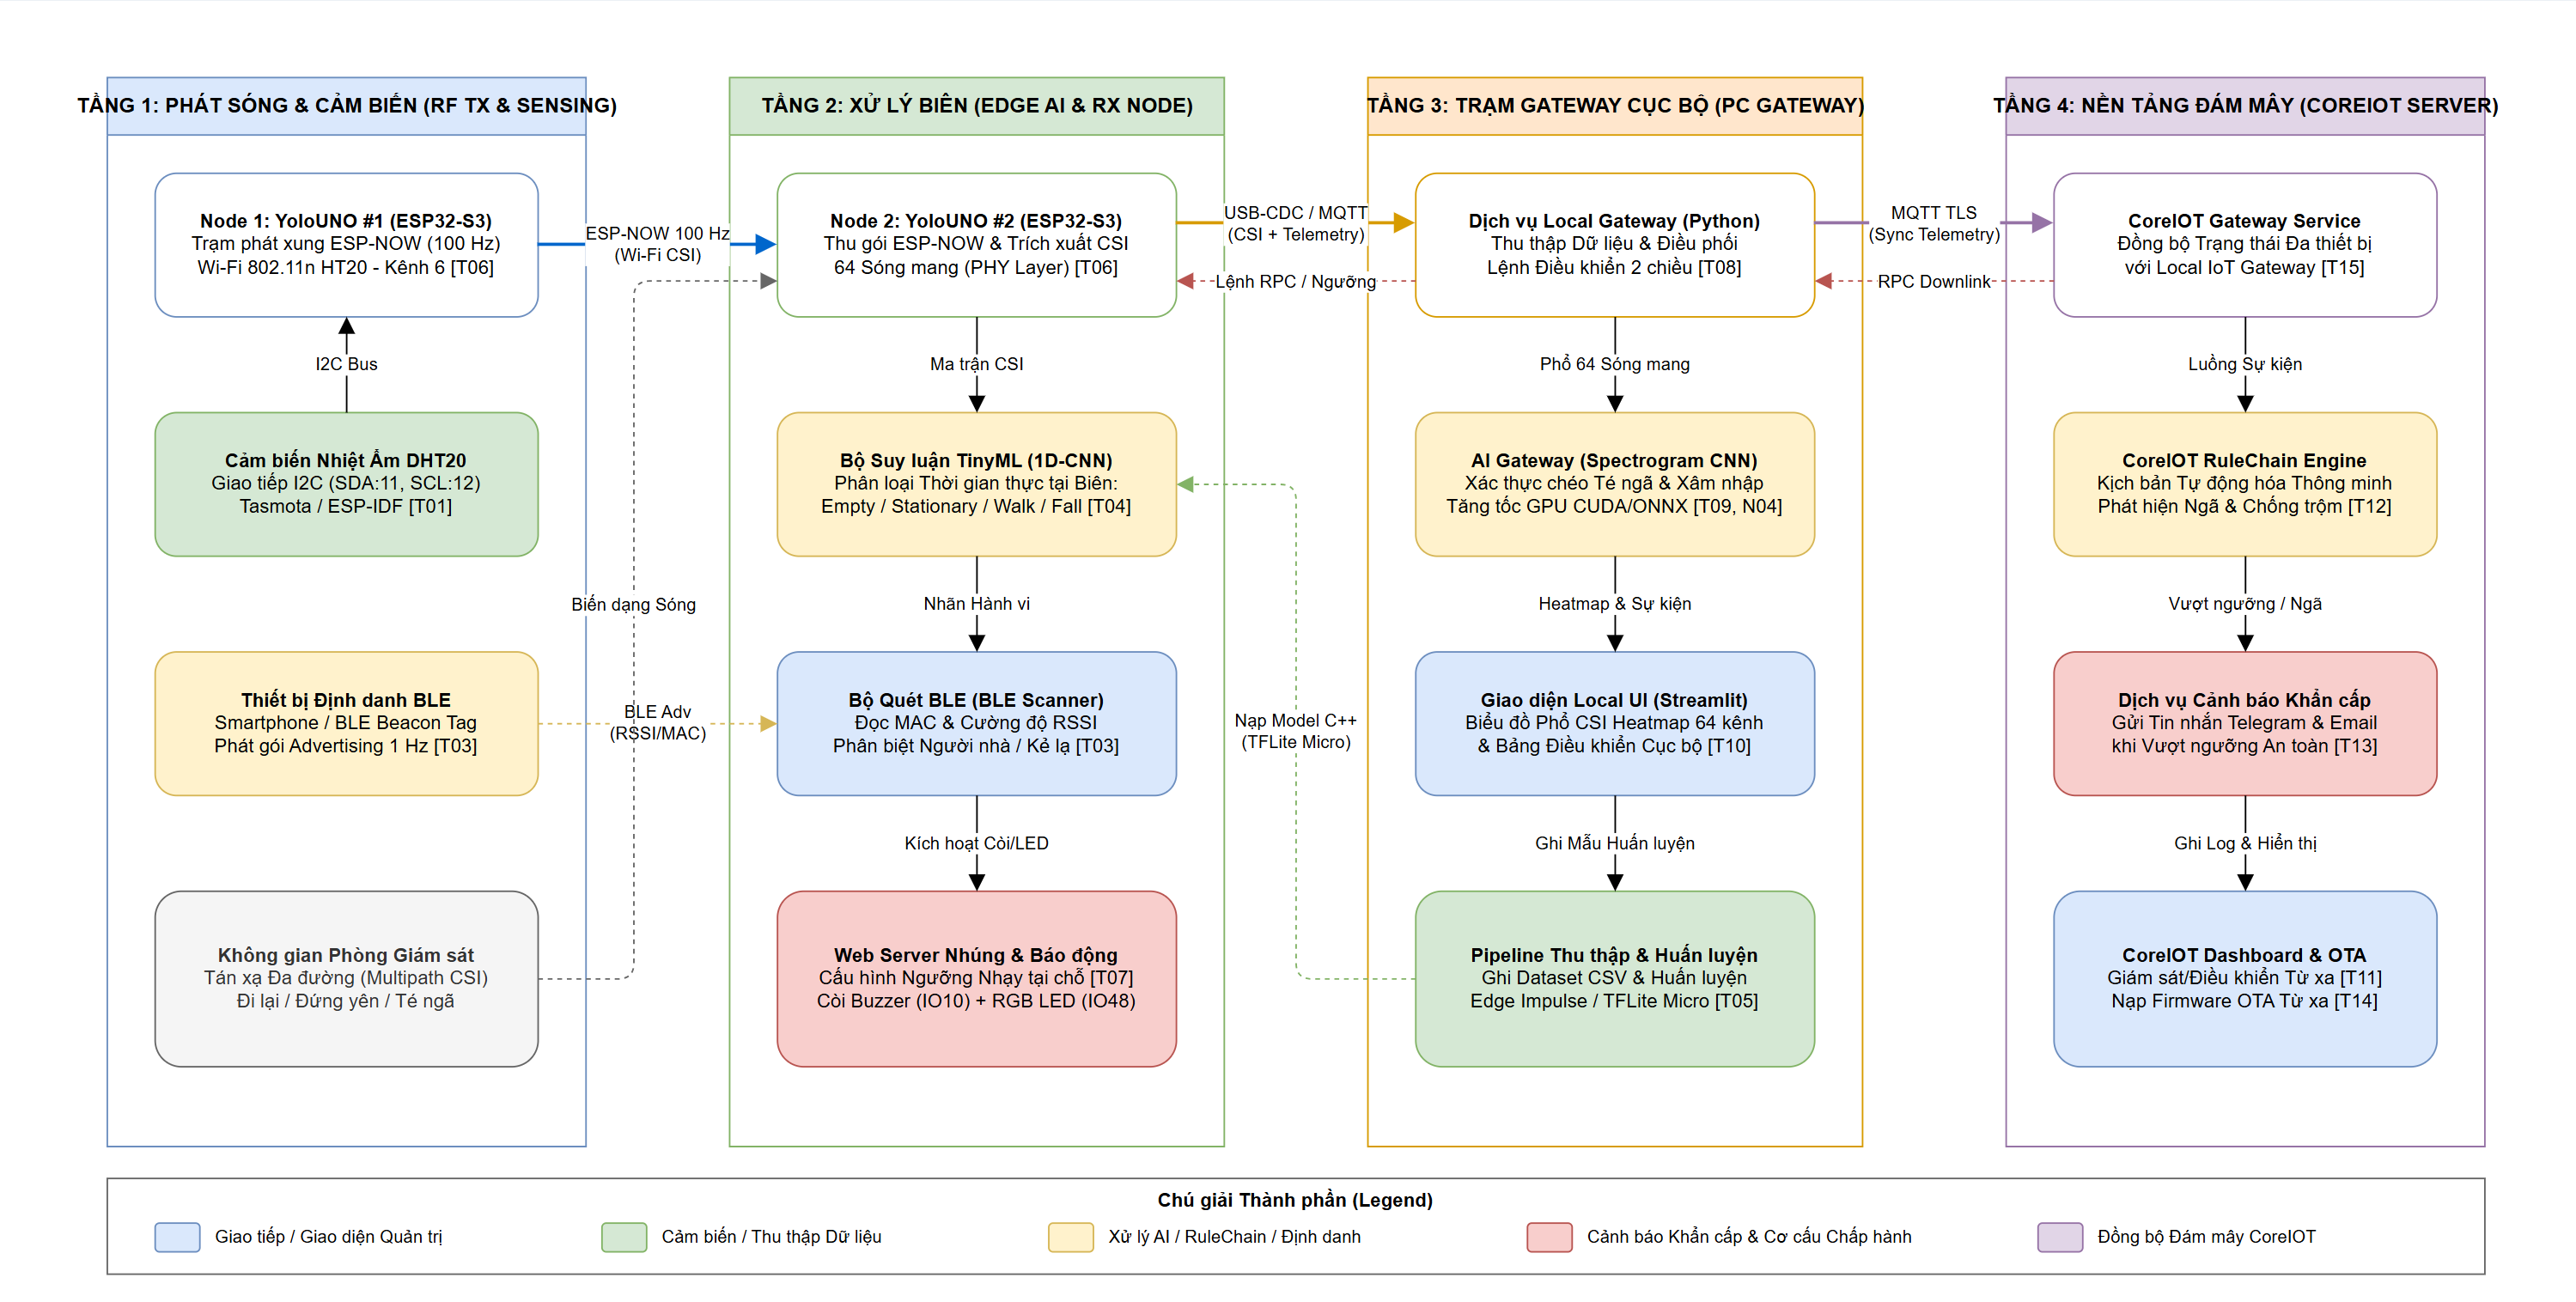
\includegraphics[width=0.98\textwidth]{graphics/drawio_overall_architecture.png}
\caption{Kiến trúc tổng thể 4 tầng của Hệ thống Radar Không Camera (Wi-Fi CSI \& BLE) Phát hiện Té ngã và Xâm nhập}
\label{fig:overall_arch}
\end{figure}

Lý do nhóm lựa chọn mô hình qua \textbf{Local IoT Gateway} kết hợp xử lý tại biên thay vì đẩy trực tiếp dữ liệu thô từ từng mạch lên đám mây gồm:
\begin{enumerate}
  \item \textbf{Giải quyết bài toán băng thông của luồng dữ liệu CSI:} Ở tần số $100\,\text{Hz}$, mỗi khung CSI gồm 64 sóng mang phức (128 byte dữ liệu I/Q) tạo ra lưu lượng liên tục khoảng $15\text{--}25\,\text{KB/s}$. Nếu bắn trực tiếp từng gói qua MQTT lên máy chủ CoreIOT từ xa sẽ gây nghẽn mạng và trễ gói. Việc truyền luồng CSI qua cổng nối tiếp tốc độ cao \texttt{USB-CDC} ($921600\,\text{bps}$) vào PC Local Gateway giúp vẽ bản đồ nhiệt thời gian thực không độ trễ (\textbf{T10}) và chỉ đẩy các bản tin tổng hợp/sự kiện đã xác thực lên CoreIOT (\textbf{T08, T15}).
  \item \textbf{Đảm bảo an toàn kép (Dual-Stage Redundancy):} Ngay cả khi mất kết nối Internet hoặc PC Gateway tắt, Node 2 vẫn tự chạy mô hình TinyML 1D-CNN nội bộ (\textbf{T04}) và kích hoạt còi báo động tại chỗ (\textbf{T07}) để cứu hộ kịp thời.
\end{enumerate}

\subsection[Sơ đồ Phân rã Chức năng]{Sơ đồ Phân rã Chức năng (Functional Decomposition)}
Toàn bộ hệ thống được phân rã thành 5 phân hệ chức năng chính tương ứng với 10 tính năng từ \textbf{F01} đến \textbf{F10} như thể hiện trên Hình \ref{fig:func_decomp}. Mỗi tính năng đều đảm nhận một khâu rõ ràng trong chuỗi thu thập $\rightarrow$ tiền xử lý $\rightarrow$ suy luận AI $\rightarrow$ hiển thị $\rightarrow$ cảnh báo và điều khiển.

\begin{figure}[H]
\centering
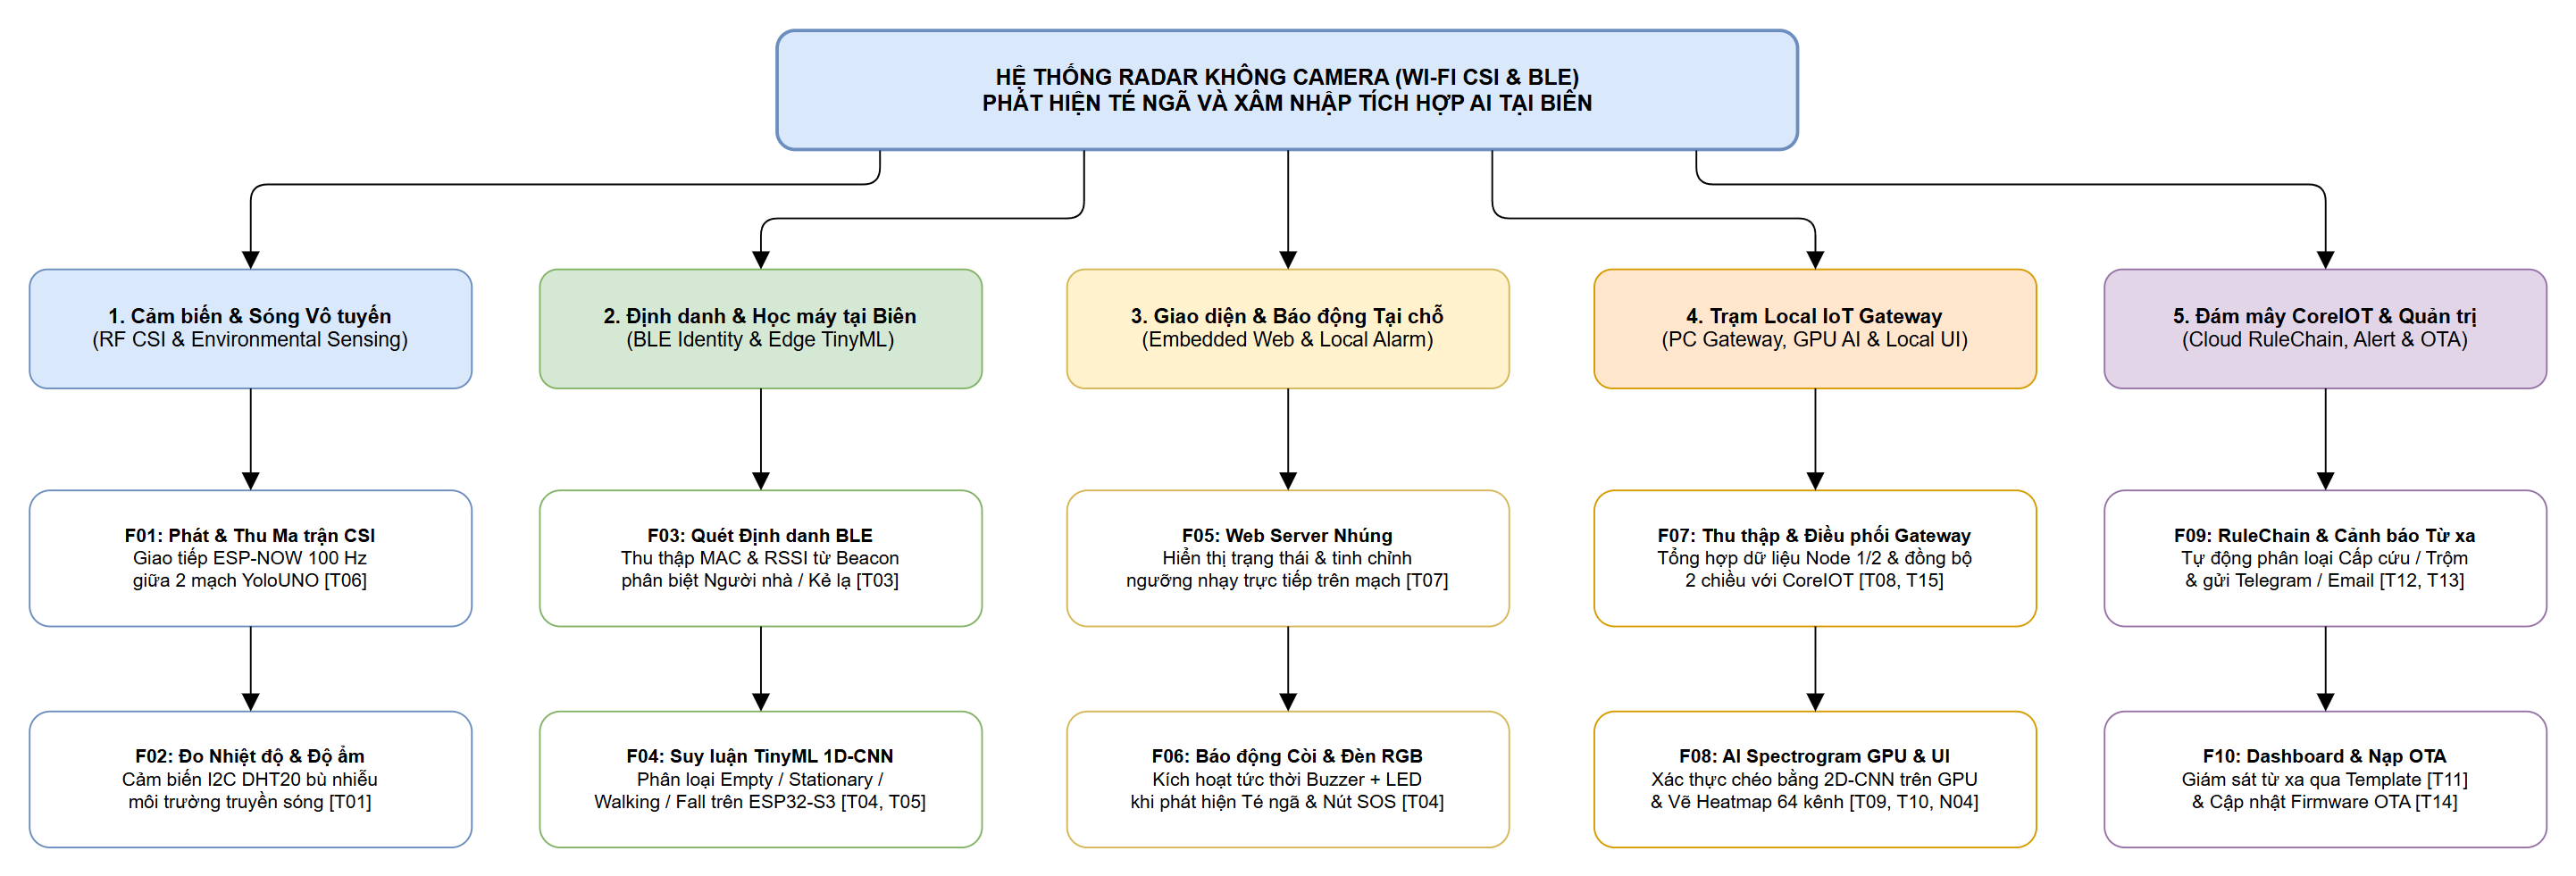
\includegraphics[width=0.98\textwidth]{graphics/drawio_functional_decomposition.png}
\caption{Sơ đồ phân rã chức năng hệ thống (Functional Decomposition Diagram) gắn với các mã công nghệ T01--T15 và N04}
\label{fig:func_decomp}
\end{figure}

\subsection[Phân tích Chi tiết các Tầng Chức năng]{Phân tích Chi tiết các Tầng Chức năng (Feature Layers)}

\subsubsection[Tầng Cảm biến và Vô tuyến (T01, T03, T06)]{Tầng Cảm biến và Thu nhận Tín hiệu Vô tuyến (Sensor Layer -- T01, T03, T06)}
Khác với các hệ thống chỉ đọc giá trị vô hướng đơn giản, tầng cảm biến của đề tài kết hợp 3 nguồn thông tin vật lý bổ trợ lẫn nhau:
\begin{itemize}
  \item \textbf{Cảm biến ma trận kênh truyền Wi-Fi CSI (\textbf{T06}):} Trên băng tần $2.4\,\text{GHz}$ chuẩn IEEE 802.11n (chế độ HT20, độ rộng kênh $20\,\text{MHz}$), tín hiệu vô tuyến được chia thành $N_{sc} = 64$ sóng mang phụ trực giao (OFDM subcarriers). Khi sóng truyền từ Node 1 (Tx) đến Node 2 (Rx) qua $L$ đường phản xạ khác nhau trong phòng (sàn nhà, tường, trần và cơ thể người), đáp ứng tần số kênh truyền phức của sóng mang thứ $k$ tại thời điểm $t$ được biểu diễn bởi phương trình:
  \begin{align}
    H_k(t) &= \sum_{l=1}^{L} \alpha_l(t) \, e^{-j 2\pi f_k \tau_l(t)} = I_k(t) + j Q_k(t) \label{eq:csi_channel}
  \end{align}
  trong đó $\alpha_l(t)$ và $\tau_l(t)$ lần lượt là hệ số suy hao biên độ và độ trễ truyền dẫn của đường thứ $l$, còn $I_k(t), Q_k(t) \in [-128, 127]$ là hai thành phần đồng pha (In-phase) và vuông pha (Quadrature) được bộ thu phần cứng của chip ESP32-S3 trích xuất trực tiếp từ trường huấn luyện dài (LLTF -- Long Training Field) của mỗi gói tin ESP-NOW. Biên độ tức thời của sóng mang thứ $k$ được tính bằng:
  \begin{align}
    |H_k(t)| &= \sqrt{I_k^2(t) + Q_k^2(t)}, \quad k \in \{1, 2, \dots, 52\} \label{eq:csi_amp}
  \end{align}
  (sau khi loại bỏ 12 sóng mang bảo vệ ở hai biên và sóng mang DC ở tâm chỉ chứa giá trị 0).
  \item \textbf{Cảm biến nhiệt độ và độ ẩm I2C DHT20 (\textbf{T01}):} Hơi nước và nhiệt độ không khí trong phòng tắm/phòng ngủ thay đổi lớn (ví dụ khi bật bình nước nóng) làm thay đổi hằng số điện môi của không khí và gây trôi nhẹ suy hao đường truyền nền. Cảm biến DHT20 giao tiếp qua chuẩn I2C (địa chỉ \texttt{0x38}, độ phân giải $0.01\,^\circ\text{C}$ và $0.024\,\%\text{RH}$) được kết nối vào Node 1 (hoặc cấu hình trên nền Tasmota/ESP-IDF) để cung cấp thông số môi trường và hiệu chuẩn ngưỡng phát hiện.
  \item \textbf{Cảm biến định danh hiện diện BLE (\textbf{T03}):} Node 2 sử dụng bộ thu Bluetooth 5.0 (LE) tích hợp trên ESP32-S3 để quét thụ động các gói tin quảng bá (\texttt{ADV\_IND}) từ thẻ khóa BLE Beacon hoặc ứng dụng phát Beacon trên điện thoại của người nhà. Khoảng cách tương đối được ước lượng từ chỉ số \texttt{RSSI} theo mô hình suy hao đường truyền logarit:
  \begin{align}
    \text{RSSI}(d) &= \text{RSSI}(d_0) - 10 \cdot n \cdot \log_{10}\left(\frac{d}{d_0}\right) + X_\sigma \label{eq:ble_rssi}
  \end{align}
  Nếu tồn tại ít nhất một địa chỉ MAC nằm trong danh sách tin cậy (\texttt{Whitelist}) có $\text{RSSI} > -75\,\text{dBm}$, hệ thống xác nhận người trong phòng là thành viên gia đình (\texttt{ble\_authorized = true}).
\end{itemize}

\subsubsection[Tầng Truyền thông (T03, T06, T08, T15)]{Tầng Truyền thông (Communication Layer -- T03, T06, T08, T15)}
Hệ thống sử dụng phân cấp truyền thông 3 chặng tối ưu hóa cho từng yêu cầu băng thông và độ trễ:
\begin{enumerate}
  \item \textbf{Chặng Node 1 $\rightarrow$ Node 2 (ESP-NOW -- T06):} Sử dụng giao thức không kết nối \textbf{ESP-NOW} của Espressif hoạt động trực tiếp ở tầng liên kết dữ liệu (Data Link Layer -- MAC) mà không cần bắt tay TCP/IP hay thông qua bộ định tuyến Wi-Fi trung gian. Tốc độ phát cố định $100\,\text{gói/giây}$ trên Kênh 6 ($2437\,\text{MHz}$), đảm bảo độ trễ truyền gói dưới $2\,\text{ms}$.
  \item \textbf{Chặng Node 2 $\leftrightarrow$ PC Local Gateway (USB-CDC Serial \& Wi-Fi):} Khung dữ liệu CSI thô và kết quả suy luận TinyML tại biên được đẩy về PC Gateway qua giao diện nối tiếp ảo tốc độ cao \texttt{USB-CDC} ($921600\,\text{bps}$) nhằm đạt thông lượng tối đa và cấp nguồn ổn định; đồng thời Node 2 vẫn duy trì kết nối Wi-Fi nội bộ để phục vụ Embedded Web Server (\textbf{T07}) và nhận bản cập nhật firmware OTA (\textbf{T14}).
  \item \textbf{Chặng PC Local Gateway $\leftrightarrow$ CoreIOT Server (MQTT Gateway API -- T08, T15):} PC Gateway kết nối lên máy chủ \texttt{app.coreiot.io} qua giao thức \textbf{MQTT} (cổng \texttt{1883} hoặc \texttt{8883} TLS), sử dụng chuẩn \textit{ThingsBoard/CoreIOT Gateway MQTT API}:
  \begin{itemize}
    \item \texttt{v1/gateway/connect}: Đăng ký tự động các thiết bị con (\texttt{YoloUNO\_Node1\_Tx}, \texttt{YoloUNO\_Node2\_Rx}) lên CoreIOT.
    \item \texttt{v1/gateway/telemetry}: Đồng bộ dữ liệu cảm biến và sự kiện AI có gắn nhãn thời gian (timestamp).
    \item \texttt{v1/gateway/attributes} \& \texttt{v1/gateway/rpc}: Đồng bộ cấu hình ngưỡng nhạy và nhận lệnh điều khiển từ xa (bật/tắt còi, đổi chế độ bảo vệ).
  \end{itemize}
\end{enumerate}

\subsubsection[Tầng Trạm Trung tâm Cục bộ (T08, T09, T10, T15)]{Tầng Trạm Trung tâm Cục bộ (Local IoT Gateway Layer -- T08, T09, T10, T15)}
Trạm Local IoT Gateway chạy trên máy tính cá nhân (PC/Laptop dùng hệ điều hành Windows/Linux) đóng vai trò là ``bộ não trung tâm tại hiện trường'' với 3 chức năng:
\begin{itemize}
  \item \textbf{Tổng hợp và điều phối dữ liệu 2 chiều (\textbf{T08}):} Đọc luồng khung tin từ Node 2, tách dữ liệu nhiệt ẩm của Node 1, dữ liệu BLE và ma trận CSI để lưu vào bộ đệm vòng (Ring Buffer) trong RAM, sau đó đóng gói JSON chuẩn hóa gửi lên CoreIOT mỗi 1 giây (hoặc gửi tức thời ngay khi có sự kiện bất thường).
  \item \textbf{Giao diện giám sát và điều khiển trực quan tại chỗ (\textbf{T10, N06}):} Xây dựng bằng \textbf{Streamlit / PyQt5} cung cấp biểu đồ bản đồ nhiệt (\textbf{Real-time CSI Heatmap}) của 52 sóng mang theo thời gian, đồ thị độ biến thiên năng lượng Doppler, trạng thái kết nối BLE, bảng nhật ký sự kiện và các nút điều khiển trực tiếp.
  \item \textbf{Đồng bộ hóa hoàn toàn với CoreIOT Gateway (\textbf{T15}):} Duy trì trạng thái \textit{Shared Attributes} và \textit{Client Attributes} đồng nhất giữa giao diện cục bộ trên PC và giao diện đám mây trên CoreIOT.
\end{itemize}

\subsubsection[Tầng Trí tuệ Nhân tạo Đa tầng (T04, T05, T09, N04)]{Tầng Trí tuệ Nhân tạo Đa tầng (Artificial Intelligence Layer -- T04, T05, T09, N04)}
Điểm đột phá kỹ thuật của đề tài là kiến trúc \textbf{AI Hiệp đồng Hai Tầng (Two-Stage Collaborative Edge-Gateway AI)}:
\begin{enumerate}
  \item \textbf{Tầng 1 -- Suy luận siêu nhẹ tại biên với TinyML (\textbf{T04, T05}):} Trên vi điều khiển ESP32-S3 của Node 2 (tích hợp bộ tập lệnh tăng tốc vector SIMD \texttt{ESP-NN} và $8\,\text{MB}$ Octal PSRAM), hệ thống gom cửa sổ trượt $T_w = 2.0\,\text{giây}$ ($200\,\text{mẫu}$), trích xuất vector đặc trưng thống kê và chạy mạng nơ-ron tích chập 1 chiều (\textbf{1D-CNN}) đã lượng tử hóa xuống số nguyên 8-bit (\texttt{INT8}). Mô hình này cho phép phát hiện sơ bộ sự kiện \texttt{Fall} hoặc \texttt{Walking} chỉ trong $<18\,\text{ms}$.
  \item \textbf{Tầng 2 -- Xác thực chéo bằng Phổ Spectrogram trên GPU Gateway (\textbf{T09, N04}):} Để loại bỏ hoàn toàn báo động giả (ví dụ khi người dùng ngồi xuống ghế nhanh hoặc làm rơi vật nặng), PC Local Gateway áp dụng phép biến đổi \textbf{STFT (Short-Time Fourier Transform)} lên chuỗi 52 sóng mang CSI để tạo ra ảnh phổ thời gian--tần số (Spectrogram kích thước $64 \times 64 \times 3$), sau đó đưa qua mạng \textbf{2D-CNN (MobileNetV2 / ResNet-18 thu gọn)} chạy trên nhân \textbf{GPU (CUDA / ONNX Runtime -- N04)} để xác thực chéo với độ chính xác vượt trội trước khi phát lệnh báo động toàn hệ thống.
\end{enumerate}

\subsubsection[Tầng Ứng dụng và Đám mây CoreIOT (T11--T14)]{Tầng Ứng dụng và Đám mây CoreIOT (Application \& Cloud Layer -- T11, T12, T13, T14)}
Trên máy chủ \textbf{CoreIOT}, hệ thống sử dụng \textbf{Device Profile \& Dashboard Template (\textbf{T11})} để hiển thị trực quan trạng thái phòng, nhiệt độ, độ ẩm, danh tính người trong phòng và lịch sử cảnh báo. Toàn bộ logic nghiệp vụ thông minh được xử lý tự động bởi \textbf{CoreIOT RuleChain (\textbf{T12})} kết hợp dịch vụ gửi tin nhắn khẩn cấp qua \textbf{Telegram Bot API và Email (\textbf{T13})}. Cuối cùng, phân hệ \textbf{OTA Firmware Repository (\textbf{T14})} trên CoreIOT quản lý các phiên bản tập tin nhị phân (\texttt{.bin}) để cập nhật từ xa cho các mạch YoloUNO.

\subsection[Bảng Ánh xạ Tính năng -- Mã Công nghệ]{Bảng Ánh xạ Tính năng -- Mã Công nghệ (Feature -- Technology Mapping)}
Bảng \ref{tab:feature_tech_mapping} ánh xạ tường minh từng tính năng \textbf{F01--F10} đã đề xuất ở Chương 1 sang các mã công nghệ \textbf{T01--T15} và \textbf{N04, N06} trong thang điểm của học phần.

\begin{table}[H]
\centering
\caption{Bảng ánh xạ hai chiều giữa các tính năng hệ thống (F01--F10) và mã công nghệ chấm điểm}
\label{tab:feature_tech_mapping}
\footnotesize
\begin{tabularx}{\textwidth}{|C{0.9cm}|Y|P{3.3cm}|P{3.6cm}|}
\hline
\textbf{Mã} & \textbf{Mô tả tóm tắt tính năng} & \textbf{Mã Công nghệ} & \textbf{Thành phần thực thi} \\
\hline
F01 & Phát/thu xung không dây tốc độ cao 100\,Hz và trích xuất ma trận 64 sóng mang Wi-Fi CSI & \textbf{T06} (1.5đ) & Node 1 (Tx) $\rightarrow$ Node 2 (Rx) \\
\hline
F02 & Giám sát nhiệt độ, độ ẩm phòng qua bus I2C để bù trừ nhiễu môi trường truyền sóng & \textbf{T01} (0.5đ) & Cảm biến DHT20 $\rightarrow$ Node 1 \\
\hline
F03 & Quét tín hiệu Bluetooth Low Energy (MAC \& RSSI) định danh chủ nhà và phát hiện người lạ & \textbf{T03} (1.5đ) & BLE Tag $\rightarrow$ Node 2 (Rx) \\
\hline
F04 & Thu thập tập dữ liệu CSV, huấn luyện và chạy mô hình TinyML 1D-CNN phân loại 4 trạng thái tại biên & \textbf{T04} (1.0đ), \textbf{T05} (1.0đ) & Edge Impulse + Node 2 (ESP32-S3) \\
\hline
F05 & Giao diện Web Server nhúng trực tiếp trên mạch cho phép cấu hình ngưỡng nhạy và điều khiển nội bộ & \textbf{T07} (1.0đ) & Node 2 (AsyncWebServer) \\
\hline
F06 & Báo động còi Buzzer, đèn WS2812B RGB tức thời tại biên và nút nhấn vật lý SOS / Hủy cảnh báo & \textbf{T04} (1.0đ), \textbf{T07} (1.0đ) & Cụm ngoại vi Node 2 \\
\hline
F07 & Dịch vụ PC Local Gateway tổng hợp dữ liệu, nhận lệnh RPC chiều về và đồng bộ với CoreIOT Gateway & \textbf{T08} (1.0đ), \textbf{T15} (2.0đ) & PC Gateway $\leftrightarrow$ CoreIOT \\
\hline
F08 & Phân tích phổ Spectrogram bằng 2D-CNN tăng tốc GPU và hiển thị bản đồ nhiệt CSI Heatmap tại chỗ & \textbf{T09} (1.0đ), \textbf{T10} (1.0đ), \textbf{N04} (1.0đ), \textbf{N06} (1.0đ) & PC Gateway (CUDA + Streamlit) \\
\hline
F09 & Kịch bản tự động hóa RuleChain phân nhánh Cấp cứu Té ngã / Báo động Trộm và gửi cảnh báo Telegram & \textbf{T12} (1.0đ), \textbf{T13} (0.5đ) & CoreIOT RuleChain + Telegram Bot \\
\hline
F10 & Thiết kế Dashboard quản trị từ xa theo Template và cập nhật Firmware OTA không dây cho ESP32-S3 & \textbf{T11} (1.0đ), \textbf{T14} (2.0đ) & CoreIOT Dashboard \& OTA Manager \\
\hline
\end{tabularx}
\end{table}

\subsection[Công nghệ Mở rộng Ngoài Danh mục]{Công nghệ Mở rộng Ngoài Danh mục (New Technologies)}
Ngoài các mã công nghệ chuẩn trong thông báo đồ án, nhóm tích hợp thêm kỹ thuật \textbf{Trích xuất và Xử lý Tín hiệu Trạng thái Kênh truyền Vô tuyến ở Tầng Vật lý (PHY-Layer Wi-Fi CSI Sensing)} dựa trên bộ thư viện \texttt{espressif/esp-csi} \cite{espressif_csi}. Thay vì chỉ sử dụng chỉ số cường độ tín hiệu tổng \texttt{RSSI} (vốn rất dễ bị nhiễu và không phản ánh được chuyển động chi tiết của tứ chi), việc khai thác đồng thời 52 sóng mang phụ OFDM cung cấp một ``ma trận cảm biến ảo'' tương đương một radar vi sai đa tần số mà không tốn thêm bất kỳ chi phí phần cứng radar nào.

\subsection[Danh mục Thiết bị Phần cứng]{Danh mục Thiết bị Phần cứng (Hardware List)}
Bảng \ref{tab:hardware_list} liệt kê chi tiết toàn bộ các thiết bị, linh kiện điện tử, chuẩn giao tiếp, số lượng và vai trò trong hệ thống.

\begin{table}[H]
\centering
\caption{Danh mục chi tiết các thiết bị phần cứng sử dụng trong hệ thống}
\label{tab:hardware_list}
\footnotesize
\begin{tabularx}{\textwidth}{|C{0.7cm}|P{3.6cm}|P{2.8cm}|C{0.7cm}|Y|}
\hline
\textbf{TT} & \textbf{Tên thiết bị / Linh kiện} & \textbf{Chuẩn giao tiếp} & \textbf{SL} & \textbf{Vai trò cụ thể trong hệ thống} \\
\hline
1 & Mạch phát triển \textbf{YoloUNO (ESP32-S3-WROOM-1)} ($16\,\text{MB}$ Flash, $8\,\text{MB}$ PSRAM) & Wi-Fi 802.11n, BLE 5.0, I2C, GPIO, USB-CDC & 02 & \textbf{Node 1 (Tx):} Phát xung ESP-NOW 100\,Hz \& đọc DHT20. \textbf{Node 2 (Rx):} Thu CSI, quét BLE, chạy TinyML, Web Server \& báo động. \\
\hline
2 & Cảm biến nhiệt độ và độ ẩm số \textbf{DHT20 (hoặc SHT30)} (Module Grove/4-pin) & I2C (\texttt{0x38}, $3.3\,\text{V}$) & 01 & Đo nhiệt độ và độ ẩm phòng chính xác cao phục vụ mã \textbf{T01} và hiệu chuẩn đường nền sóng CSI. \\
\hline
3 & Thiết bị phát định danh \textbf{BLE Beacon Tag} (hoặc Smartphone chạy nRF Connect) & BLE 5.0 Advertising ($2.4\,\text{GHz}$) & 01 & Phát khung nhận dạng MAC và UUID định kỳ để Node 2 xác thực danh tính người nhà (\textbf{T03}). \\
\hline
4 & Module còi báo động \textbf{KY-012 Active/PWM Buzzer} (kèm Transistor kích dòng) & Digital GPIO / PWM (\texttt{GPIO10}, $5\,\text{V}$) & 01 & Phát âm thanh báo động khẩn cấp tại chỗ ($85\,\text{dB}$) khi phát hiện người té ngã hoặc kẻ gian đột nhập. \\
\hline
5 & Cụm đèn LED địa chỉ hóa \textbf{WS2812B NeoPixel RGB} (4 bóng + LED onboard) & Single-wire NZR (\texttt{GPIO18 / GPIO48}) & 01 & Hiển thị trực quan trạng thái: Xanh lá (An toàn), Vàng (Có người đi lại), Đỏ chớp (Té ngã / Báo động). \\
\hline
6 & Module nút nhấn \textbf{Tactile Push Button} (kèm mạch chống dội RC) & Digital Input Pull-up (\texttt{GPIO14}) & 01 & Cho phép người dùng nhấn đơn để hủy báo động giả, hoặc nhấn giữ 3 giây để kích hoạt báo động SOS. \\
\hline
7 & Máy tính cá nhân \textbf{PC / Laptop} tích hợp GPU rời NVIDIA (hỗ trợ CUDA) & USB-CDC ($921600\,\text{bps}$), Wi-Fi, MQTT TLS & 01 & Đóng vai trò \textbf{Local IoT Gateway (\textbf{T08})}, chạy giao diện Local UI (\textbf{T10}) và mô hình AI 2D-CNN trên GPU (\textbf{T09, N04}). \\
\hline
8 & Cáp dữ liệu \textbf{USB Type-C} chống nhiễu, Breadboard và dây cắm Jumper & Nguồn $5\,\text{V DC}$ \& USB Serial & 02 & Cấp nguồn ổn định cho 2 mạch YoloUNO và truyền luồng dữ liệu CSI tốc độ cao về PC Gateway. \\
\hline
\end{tabularx}
\end{table}

% =========================================================================
% CHUONG 3: DAC TA TRIEN KHAI HE THONG VA SO DO CAM MACH
% =========================================================================
\section[Đặc tả Triển khai Hệ thống và Sơ đồ Cắm mạch]{Đặc tả Triển khai Hệ thống và Sơ đồ Cắm mạch (System Implementation)}

\subsection[Sơ đồ Đấu nối Phần cứng Chi tiết]{Sơ đồ Đấu nối Phần cứng Chi tiết (Hardware and Wiring Diagrams)}
Để việc lắp ráp mạch thực tế trên Breadboard hoặc cổng mở rộng của mạch \textbf{YoloUNO (ESP32-S3)} diễn ra chính xác tuyệt đối, tránh chạm chập nguồn hoặc xung đột chân chức năng đặc biệt (strapping pins) của chip ESP32-S3, Hình \ref{fig:hw_wiring} trình bày sơ đồ nguyên lý đấu nối chi tiết của cả hai cụm thiết bị: \textbf{Cụm Node 1 (Trạm phát sóng CSI \& Cảm biến môi trường)} và \textbf{Cụm Node 2 (Trạm thu Radar CSI, Quét BLE \& Edge AI)}.

\begin{figure}[H]
\centering
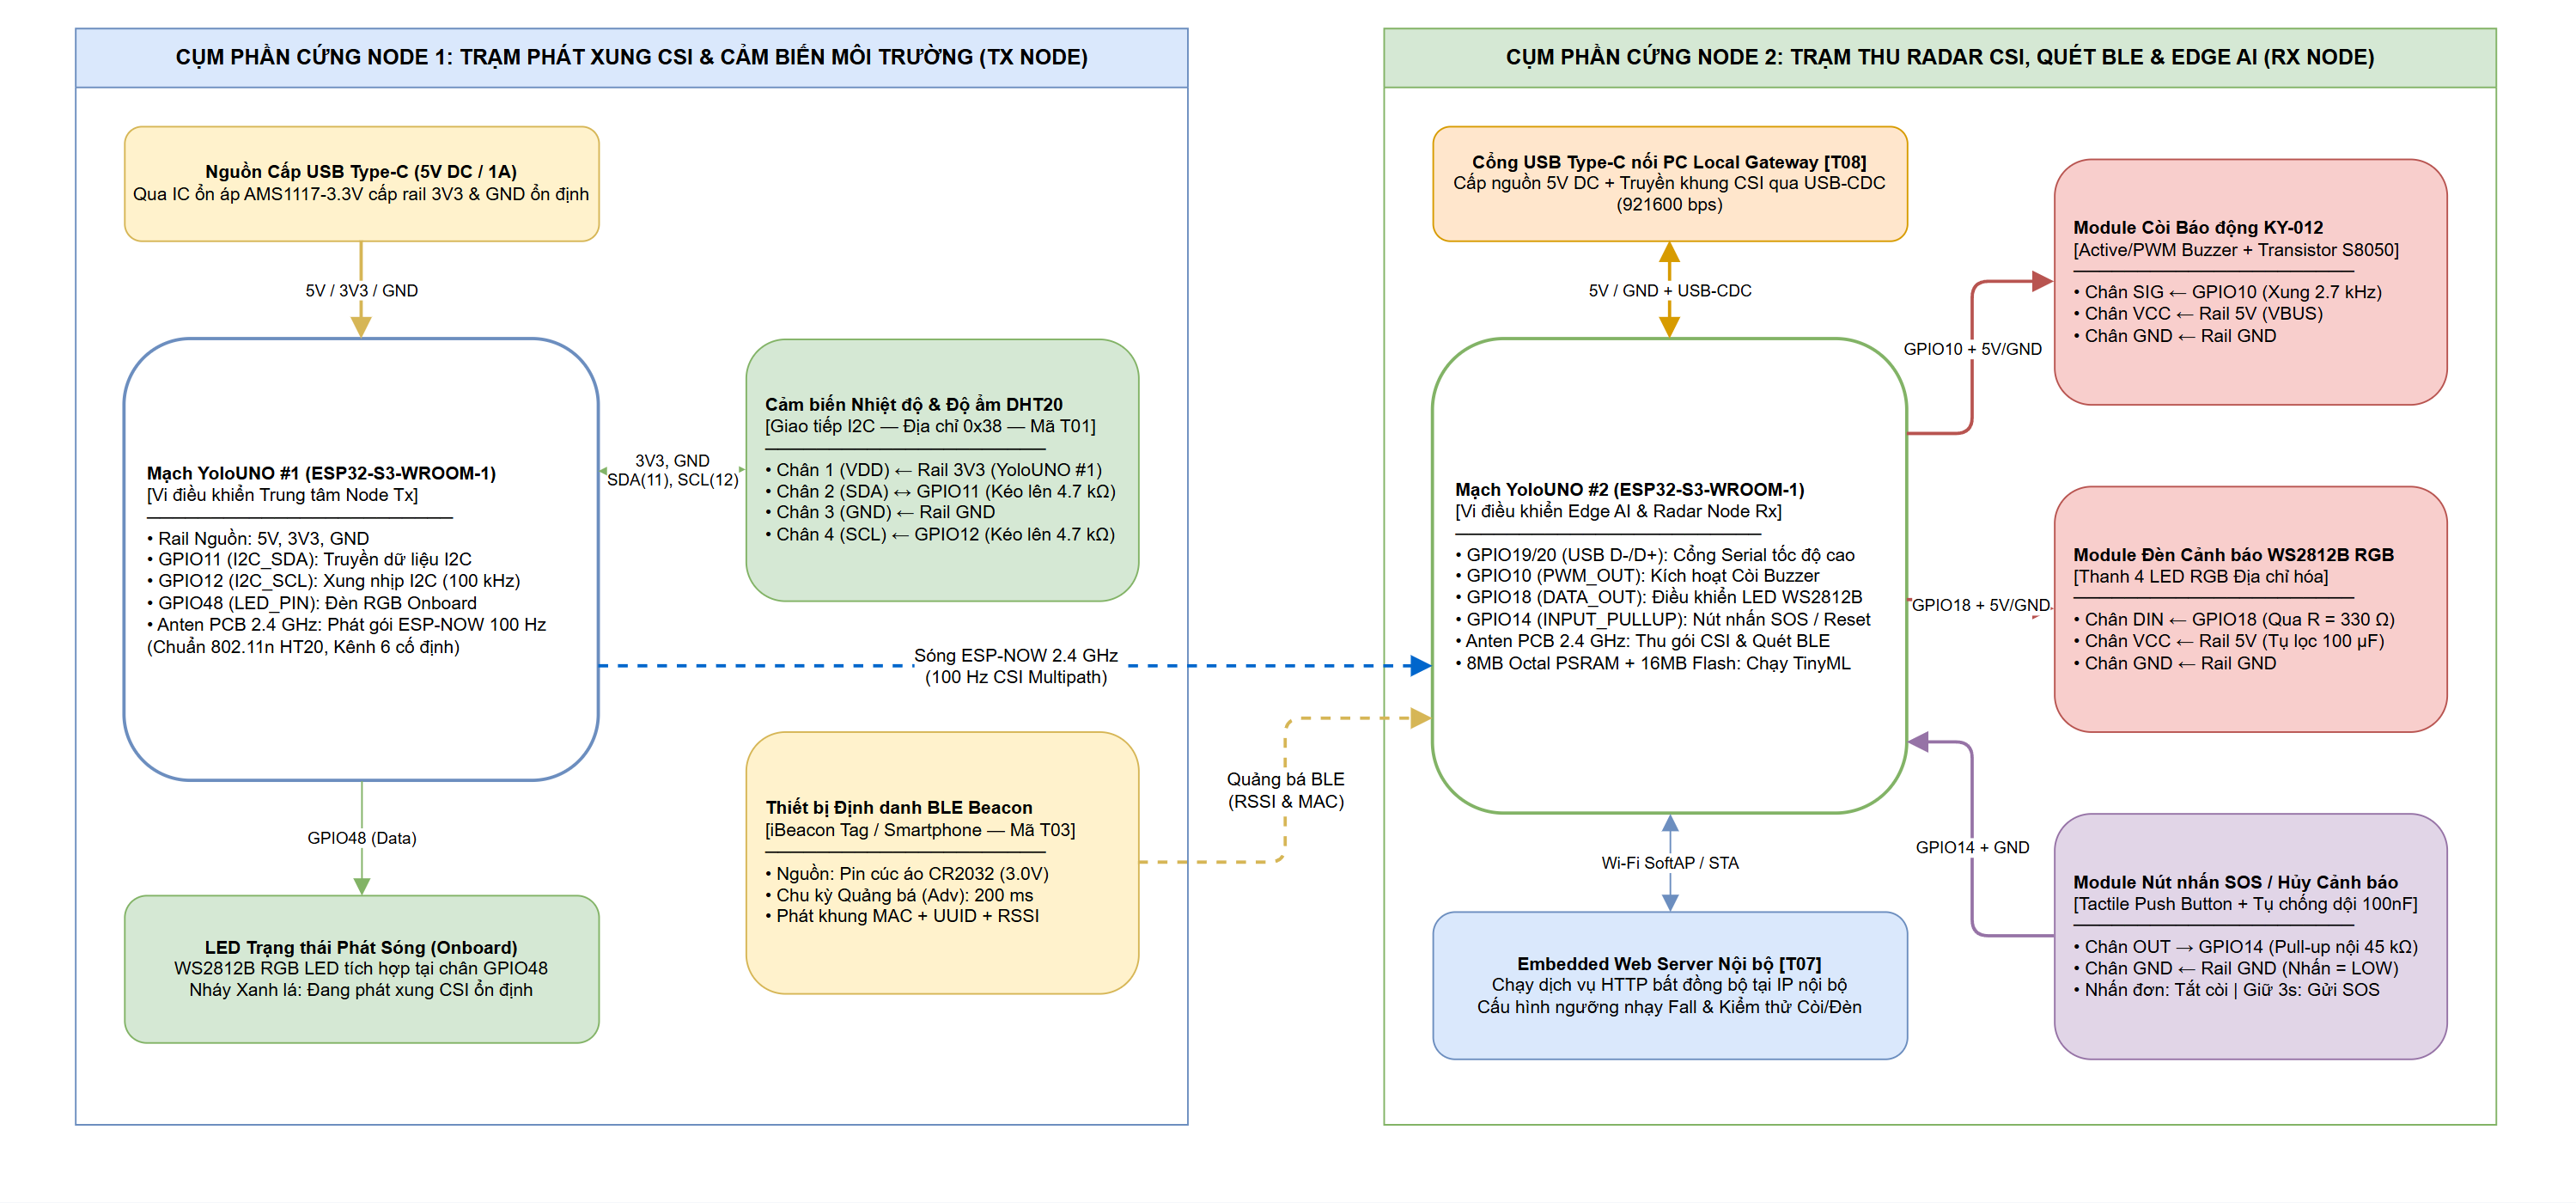
\includegraphics[width=0.98\textwidth]{graphics/drawio_hardware_wiring.png}
\caption{Sơ đồ đấu nối phần cứng chi tiết (Pinout \& Wiring Diagram) của Cụm Node 1 (Tx) và Cụm Node 2 (Rx)}
\label{fig:hw_wiring}
\end{figure}

Bảng \ref{tab:pinout_node1} và Bảng \ref{tab:pinout_node2} quy định chi tiết sơ đồ cắm từng dây dẫn (Pin-to-Pin Mapping), mức điện áp hoạt động và lưu ý kỹ thuật khi lắp mạch.

\begin{table}[H]
\centering
\caption{Bảng sơ đồ cắm mạch chi tiết cho Cụm Node 1 -- Trạm Phát sóng \& Cảm biến I2C (YoloUNO \#1)}
\label{tab:pinout_node1}
\footnotesize
\begin{tabularx}{\textwidth}{|P{2.8cm}|P{2.2cm}|P{2.6cm}|C{1.8cm}|Y|}
\hline
\textbf{Linh kiện ngoại vi} & \textbf{Chân ngoại vi} & \textbf{Chân YoloUNO \#1} & \textbf{Mức áp} & \textbf{Chức năng \& Lưu ý đấu nối kỹ thuật} \\
\hline
\multirow{4}{=}{\textbf{Cảm biến DHT20 (I2C)}} & Chân 1 (\texttt{VDD}) & Chân \texttt{3V3} & $3.3\,\text{V DC}$ & Cấp nguồn logic $3.3\,\text{V}$ ổn định từ IC LDO trên mạch YoloUNO. \\
\cline{2-5}
 & Chân 2 (\texttt{SDA}) & \texttt{GPIO11} (\texttt{SDA}) & $3.3\,\text{V TTL}$ & Đường dữ liệu I2C hai chiều (module đã có sẵn trở kéo lên $4.7\,\text{k}\Omega$). \\
\cline{2-5}
 & Chân 3 (\texttt{GND}) & Chân \texttt{GND} & $0\,\text{V}$ (Mass) & Nối đất chung với mạch YoloUNO \#1. \\
\cline{2-5}
 & Chân 4 (\texttt{SCL}) & \texttt{GPIO12} (\texttt{SCL}) & $3.3\,\text{V TTL}$ & Đường xung nhịp I2C tốc độ tiêu chuẩn $100\,\text{kHz}$. \\
\hline
\textbf{LED RGB Onboard} & \texttt{DIN} (Nội mạch) & \texttt{GPIO48} & $3.3\,\text{V TTL}$ & Đèn WS2812B tích hợp sẵn trên YoloUNO; nháy xanh lá báo đang phát ESP-NOW. \\
\hline
\textbf{Nguồn cấp USB-C} & \texttt{VBUS / GND} & Cổng \texttt{USB-C} & $5.0\,\text{V} / 1\,\text{A}$ & Cấp nguồn từ củ sạc $5\,\text{V}$ hoặc pin dự phòng đặt cố định ở góc phòng đối diện Node 2. \\
\hline
\end{tabularx}
\end{table}

\begin{table}[H]
\centering
\caption{Bảng sơ đồ cắm mạch chi tiết cho Cụm Node 2 -- Trạm Thu Radar CSI, BLE \& Edge AI (YoloUNO \#2)}
\label{tab:pinout_node2}
\footnotesize
\begin{tabularx}{\textwidth}{|P{2.8cm}|P{2.2cm}|P{2.6cm}|C{1.8cm}|Y|}
\hline
\textbf{Linh kiện ngoại vi} & \textbf{Chân ngoại vi} & \textbf{Chân YoloUNO \#2} & \textbf{Mức áp} & \textbf{Chức năng \& Lưu ý đấu nối kỹ thuật} \\
\hline
\multirow{3}{=}{\textbf{Còi Buzzer KY-012}} & Chân \texttt{SIG} (\texttt{I/O}) & \texttt{GPIO10} & $3.3\,\text{V PWM}$ & Xuất xung PWM tần số $2.7\,\text{kHz}$ kích cực B của Transistor S8050 trên module còi. \\
\cline{2-5}
 & Chân \texttt{VCC} (\texttt{+}) & Chân \texttt{5V} (\texttt{VBUS}) & $5.0\,\text{V DC}$ & Cấp nguồn $5\,\text{V}$ để còi đạt âm lượng lớn nhất ($\approx 85\,\text{dB}$). \\
\cline{2-5}
 & Chân \texttt{GND} (\texttt{-}) & Chân \texttt{GND} & $0\,\text{V}$ (Mass) & Nối đất chung của hệ thống. \\
\hline
\multirow{3}{=}{\textbf{Đèn WS2812B RGB}} & Chân \texttt{DIN} & \texttt{GPIO18} & $3.3\,\text{V TTL}$ & Nối qua điện trở hạn dòng $330\,\Omega$ để bảo vệ chân dữ liệu đầu vào của LED đầu tiên. \\
\cline{2-5}
 & Chân \texttt{VCC} (\texttt{+5V}) & Chân \texttt{5V} (\texttt{VBUS}) & $5.0\,\text{V DC}$ & Mắc song song tụ hóa $100\,\mu\text{F}/16\,\text{V}$ giữa \texttt{5V} và \texttt{GND} để chống sụt áp khi LED sáng đỏ tối đa. \\
\cline{2-5}
 & Chân \texttt{GND} & Chân \texttt{GND} & $0\,\text{V}$ (Mass) & Nối đất chung. \\
\hline
\multirow{2}{=}{\textbf{Nút nhấn SOS / Reset}} & Chân \texttt{OUT} (Chân 1) & \texttt{GPIO14} & $3.3\,\text{V TTL}$ & Cấu hình \texttt{INPUT\_PULLUP} nội bộ ($45\,\text{k}\Omega$); bình thường ở mức \texttt{HIGH}, khi nhấn xuống mức \texttt{LOW}. \\
\cline{2-5}
 & Chân \texttt{GND} (Chân 2) & Chân \texttt{GND} & $0\,\text{V}$ (Mass) & Mắc song song tụ gốm $100\,\text{nF}$ giữa \texttt{GPIO14} và \texttt{GND} để khử nhiễu dội phím phần cứng. \\
\hline
\textbf{Cổng USB Type-C} & \texttt{USB D- / D+} & \texttt{GPIO19 / GPIO20} & $5.0\,\text{V} / \text{USB}$ & Cắm trực tiếp vào PC Local Gateway: vừa cấp nguồn $5\,\text{V}$, vừa truyền luồng CSI tốc độ $921600\,\text{bps}$. \\
\hline
\end{tabularx}
\end{table}

\subsection[Đặc tả Thiết kế Firmware trên Thiết bị]{Đặc tả Thiết kế Firmware trên Thiết bị (Device Firmware)}

\subsubsection[Firmware Node 1 -- Trạm Phát CSI và I2C (T01, T06)]{Thiết kế Firmware Node 1 -- Trạm Phát sóng CSI và Cảm biến I2C (T01, T06)}
Node 1 có thể vận hành linh hoạt ở hai chế độ: (1) Chạy firmware \textbf{Tasmota} tích hợp sẵn trình điều khiển I2C đọc cảm biến DHT20/SHT30 xuất chuỗi JSON định kỳ (\textbf{T01}); hoặc (2) Chạy firmware chuyên dụng biên dịch trên nền \textbf{ESP-IDF v5.1 / PlatformIO} kết hợp đọc I2C DHT20 và bộ định thời phần cứng (\texttt{esp\_timer}) phát gói tin \textbf{ESP-NOW} đúng chu kỳ $\Delta t = 10\,\text{ms}$ ($100\,\text{Hz}$). Trên hệ điều hành thời gian thực \textbf{FreeRTOS} của ESP32-S3, Node 1 khởi tạo 2 tác vụ độc lập:
\begin{itemize}
  \item \texttt{Task\_I2C\_EnvRead} (Core 0, Độ ưu tiên 3, Chu kỳ $5000\,\text{ms}$): Giao tiếp với địa chỉ \texttt{0x38} trên bus I2C (\texttt{GPIO11/12}), kích hoạt lệnh đo \texttt{0xAC 0x33 0x00}, đọc 7 byte dữ liệu trả về, kiểm tra mã vòng \texttt{CRC-8} và quy đổi ra giá trị thực $T\,(^\circ\text{C})$, $RH\,(\%)$.
  \item \texttt{Task\_ESPNOW\_PingTx} (Core 1, Độ ưu tiên 10, Chu kỳ $10\,\text{ms}$): Cố định kênh vô tuyến Wi-Fi ở Kênh 6, tắt chế độ tiết kiệm năng lượng modem (\texttt{esp\_wifi\_set\_ps(WIFI\_PS\_NONE)}) để giữ công suất phát ổn định ở mức $+19.5\,\text{dBm}$, và phát liên tục khung tin \texttt{csi\_ping\_packet\_t} tới địa chỉ MAC của Node 2.
\end{itemize}

\subsubsection[Firmware Node 2 -- Trạm Thu CSI, BLE và TinyML (T03, T04, T06)]{Thiết kế Firmware Node 2 -- Trạm Thu Radar CSI, BLE và TinyML (T03, T04, T06)}
Trên Node 2 (YoloUNO \#2), để tránh việc quét BLE và xử lý mạng làm gián đoạn luồng ngắt thu CSI ở tầng vật lý, kiến trúc phần mềm được phân bổ chặt chẽ lên 2 nhân xử lý Xtensa LX7 ($240\,\text{MHz}$) của chip ESP32-S3:
\begin{itemize}
  \item \textbf{Hàm gọi lại tầng phần cứng \texttt{wifi\_csi\_rx\_cb()} (Chạy trong ngữ cảnh IRAM):} Đăng ký qua API \texttt{esp\_wifi\_set\_csi\_rx\_cb()}. Ngay khi phần cứng RF giải điều chế xong một khung ESP-NOW từ địa chỉ MAC của Node 1, hàm này chép mảng $128\,\text{byte}$ dữ liệu phức $I/Q$ cùng giá trị \texttt{rx\_ctrl.rssi} và \texttt{timestamp} đẩy vào hàng đợi không khóa \texttt{xQueueCSI} (sức chứa 64 khung trong PSRAM).
  \item \textbf{\texttt{Task\_CSI\_TinyML} (Ghim trên Core 1 -- Nhân chuyên dụng DSP/AI, Độ ưu tiên 12):} Lấy khung CSI từ \texttt{xQueueCSI}, tính biên độ 52 sóng mang theo công thức (\ref{eq:csi_amp}), áp dụng bộ lọc trung vị trượt Hampel ($k=5$) và bộ lọc thông dải IIR Butterworth bậc 4 ($0.2\text{--}15\,\text{Hz}$). Mỗi $200\,\text{ms}$ (bước trượt 20 mẫu trên cửa sổ 200 mẫu), tác vụ gọi bộ thông dịch \textbf{TensorFlow Lite Micro} thực thi mô hình \texttt{1D-CNN INT8} để cập nhật nhãn hành vi tại biên và xuất luồng khung dữ liệu ra cổng \texttt{USB-CDC} về PC Gateway.
  \item \textbf{\texttt{Task\_BLE\_Scanner} (Ghim trên Core 0, Độ ưu tiên 5):} Sử dụng ngăn xếp \textbf{NimBLE} nhẹ hơn Bluedroid 50\% RAM, mở cửa sổ quét thụ động (\texttt{Passive Scan}) thời lượng $80\,\text{ms}$ mỗi chu kỳ $1000\,\text{ms}$ để cập nhật bảng hiện diện của các thẻ BLE Beacon mà không gây xung đột bộ chia sẻ ăng-ten Wi-Fi/BLE (\texttt{Coexistence Arbitrator}).
\end{itemize}

\subsubsection[Embedded Web Server Nội bộ trên Node 2 (T07)]{Thiết kế Embedded Web Server Nội bộ trên Node 2 (T07)}
Nhằm đáp ứng trọn vẹn mã công nghệ \textbf{T07 (1.0 điểm)}, Node 2 khởi chạy một máy chủ HTTP bất đồng bộ (\texttt{ESPAsyncWebServer}) tại cổng \texttt{80}. Giao diện Web nhúng được viết bằng HTML5/CSS/JavaScript gọn nhẹ lưu trong phân vùng bộ nhớ \texttt{LittleFS}, giao tiếp với vi điều khiển qua 3 điểm cuối RESTful API và WebSocket:
\begin{itemize}
  \item \texttt{GET /api/status}: Trả về chuỗi JSON chứa trạng thái hiện tại (\texttt{EMPTY}, \texttt{STATIONARY}, \texttt{WALKING}, \texttt{FALL}), xác suất tin cậy của TinyML, nhiệt độ/độ ẩm từ Node 1, trạng thái định danh BLE và địa chỉ IP.
  \item \texttt{POST /api/config}: Cho phép người dùng tinh chỉnh trực tiếp ngưỡng độ nhạy phát hiện ngã (\texttt{fall\_threshold} $\in [0.50, 0.95]$), ngưỡng cường độ BLE (\texttt{ble\_rssi\_min}) và bật/tắt chế độ chống trộm (\texttt{security\_armed}).
  \item \texttt{POST /api/alarm}: Cho phép bật/tắt cưỡng bức còi Buzzer (\texttt{GPIO10}) và đổi màu đèn NeoPixel (\texttt{GPIO18}) để kiểm thử phần cứng tại chỗ.
\end{itemize}

\subsection[Giao thức Truyền thông ESP-NOW và BLE (T03, T06)]{Đặc tả Giao thức Truyền thông Giữa các Thiết bị (ESP-NOW \& BLE -- T03, T06)}
Để tối ưu hóa hiệu quả truyền dẫn và chống nhiễu gói tin từ các mạng Wi-Fi xung quanh, nhóm định nghĩa cấu trúc khung gói tin nhị phân \texttt{csi\_ping\_packet\_t} có kích thước cố định $24\,\text{byte}$ truyền qua giao thức \textbf{ESP-NOW} như trong Đoạn mã \ref{lst:espnow_struct}.

\begin{lstlisting}[language=C++, caption={Cấu trúc khung tin ESP-NOW (T06) và hàm callback trích xuất ma trận CSI trên ESP32-S3}, label={lst:espnow_struct}]
#pragma pack(push, 1)
typedef struct {
    uint16_t magic_header;   // Co dinh 0xC51A de loc dung goi cua he thong
    uint32_t seq_id;         // So thu tu goi tang dan (kiem tra mat goi)
    uint32_t tx_time_ms;     // Nhan thoi gian phat tu Node 1 (ms)
    float    temp_c;         // Nhiet do doc tu cam bien I2C DHT20 (T01)
    float    humi_rh;        // Do am tuong doi tu cam bien I2C DHT20 (T01)
    uint8_t  tx_status_flag; // Co trang thai cua Node 1
    uint8_t  crc8_checksum;  // Ma kiem tra loi CRC-8 da thuc 0x07
} csi_ping_packet_t;
#pragma pack(pop)

static void IRAM_ATTR wifi_csi_rx_cb(void *ctx, wifi_csi_info_t *info) {
    if (!info || !info->buf || info->len < 128) return;
    // Chi nhan goi CSI xuat phat tu dia chi MAC cua Node 1 (Tx)
    if (memcmp(info->mac, NODE1_TX_MAC_ADDR, 6) != 0) return;

    csi_frame_item_t item;
    item.timestamp_us = esp_timer_get_time();
    item.rssi         = info->rx_ctrl.rssi;
    item.noise_floor  = info->rx_ctrl.noise_floor;
    memcpy(item.iq_raw, info->buf, 128); // 64 subcarriers * 2 bytes (I, Q)
    xQueueSendFromISR(xQueueCSI, &item, NULL);
}
\end{lstlisting}

\subsection[Đặc tả Trạm Local IoT Gateway trên PC (T08, T10, T15)]{Đặc tả Trạm Local IoT Gateway trên PC (T08, T10, T15)}
Ứng dụng \textbf{PC Local IoT Gateway} được kiến trúc theo mô hình đa luồng bất đồng bộ bằng ngôn ngữ \textbf{Python 3.11}, bao gồm 3 mô-đun cốt lõi:
\begin{enumerate}
  \item \textbf{Mô-đun Thu thập và Phân phối Lệnh (\texttt{gateway\_core.py} -- T08):} Mở luồng đọc cổng nối tiếp \texttt{pyserial} ở tốc độ $921600\,\text{bps}$, giải mã khung dữ liệu từ Node 2, cập nhật vào cơ sở dữ liệu thời gian thực trong bộ nhớ (SQLite / In-memory Queue) và lắng nghe các lệnh điều khiển RPC từ đám mây CoreIOT để chuyển tiếp tức thời xuống Node 2 qua cổng Serial hoặc HTTP.
  \item \textbf{Mô-đun Đồng bộ CoreIOT Gateway (\texttt{coreiot\_sync.py} -- T15):} Sử dụng thư viện \texttt{paho-mqtt} kết nối tới máy chủ \texttt{app.coreiot.io} dưới danh nghĩa một thiết bị kiểu \textbf{Gateway} (\texttt{IsGateway = true}). Khi khởi động, chương trình tự động gửi gói đăng ký 2 thiết bị con (\texttt{Node1\_Env\_Tx} và \texttt{Node2\_Radar\_Rx}) lên CoreIOT, đồng bộ hóa hai chiều các thuộc tính cấu hình (\texttt{fall\_threshold}, \texttt{security\_mode}, \texttt{firmware\_version}) và đẩy gói JSON Telemetry định kỳ.
  \item \textbf{Mô-đun Giao diện Giám sát Cục bộ (\texttt{local\_ui.py} -- T10, N06):} Xây dựng bằng \textbf{Streamlit} (hoặc \textbf{PyQt5}), hiển thị trực tiếp đồ thị sóng mang 64 kênh nhảy múa theo thời gian thực, bản đồ nhiệt phổ tần số Spectrogram, chỉ báo định danh BLE, cùng bảng nút bấm điều khiển còi báo động và ghi nhãn dữ liệu huấn luyện (\textbf{T05}).
\end{enumerate}

\subsection[Đặc tả Pipeline Trí tuệ Nhân tạo Đa tầng (T04, T05, T09, N04)]{Đặc tả Pipeline Trí tuệ Nhân tạo Đa tầng (T04, T05, T09, N04)}
Hình \ref{fig:ai_pipeline} trình bày lưu đồ xử lý toàn diện từ lúc thu nhận sóng CSI thô ở tầng vật lý cho đến khi suy luận qua hai tầng AI (TinyML trên ESP32-S3 và Spectrogram 2D-CNN trên GPU của PC Gateway) và kích hoạt kịch bản tự động hóa trên CoreIOT RuleChain.

\begin{figure}[H]
\centering
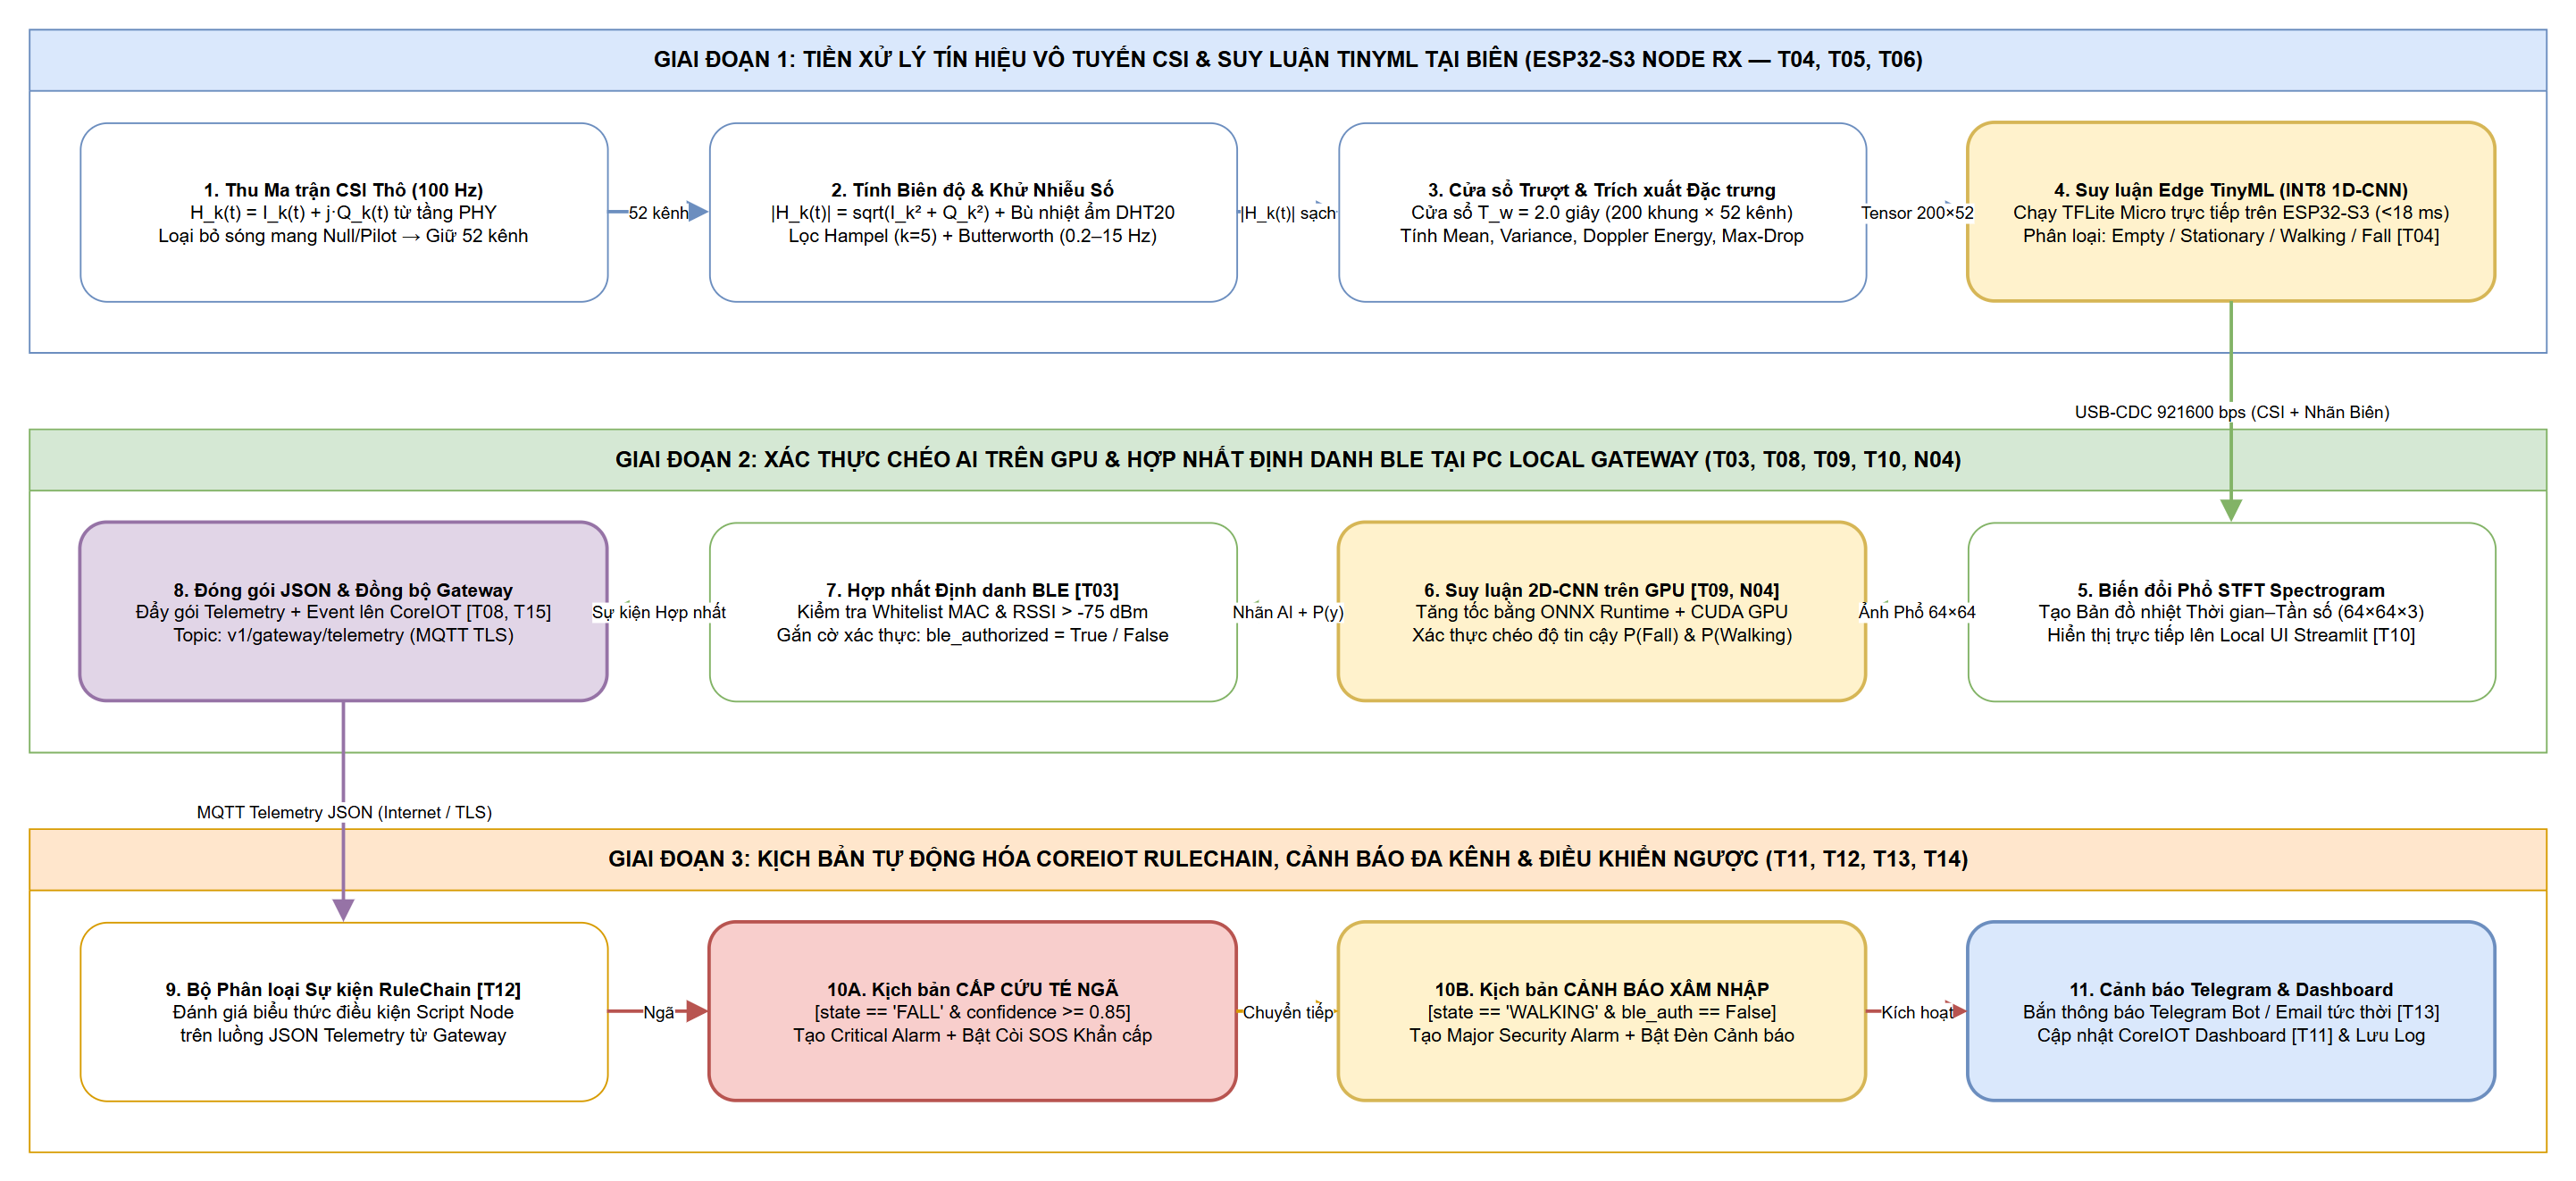
\includegraphics[width=0.98\textwidth]{graphics/drawio_ai_rulechain_pipeline.png}
\caption{Lưu đồ thuật toán xử lý tín hiệu CSI, suy luận AI đa tầng (TinyML + GPU Gateway) và kịch bản CoreIOT RuleChain}
\label{fig:ai_pipeline}
\end{figure}

\subsubsection[Thu thập Dữ liệu và Tiền xử lý (T05)]{Quy trình Thu thập Dữ liệu và Tiền xử lý (Data Collection \& Preprocessing -- T05)}
Để xây dựng bộ dữ liệu chất lượng cao phục vụ mã \textbf{T05 (1.0 điểm)}, nhóm xây dựng công cụ tự động \texttt{tools/csi\_collector.py} cho phép thu thập và gắn nhãn các cửa sổ tín hiệu dài $2.0\,\text{giây}$ ($200\,\text{khung} \times 52\,\text{sóng mang}$) cho 4 lớp hành vi:
\begin{enumerate}
  \item \textbf{Lớp 0 -- \texttt{EMPTY} (Phòng trống):} Không có người trong phòng; biên độ các sóng mang phẳng, phương sai trung bình $\bar{\sigma}^2 < 0.35$.
  \item \textbf{Lớp 1 -- \texttt{STATIONARY} (Đứng yên / Ngồi / Thở):} Có người ngồi đọc sách hoặc nằm ngủ; xuất hiện dao động tuần hoàn biên độ nhỏ ở tần số nhịp thở $0.2\text{--}0.5\,\text{Hz}$.
  \item \textbf{Lớp 2 -- \texttt{WALKING} (Đi lại bình thường):} Người di chuyển trong phòng; tạo ra hiệu ứng dịch tần Doppler làm các sóng mang biến thiên nhịp nhàng ở dải tần $1.0\text{--}4.0\,\text{Hz}$.
  \item \textbf{Lớp 3 -- \texttt{FALL} (Té ngã đột ngột):} Cơ thể rơi tự do xuống sàn trong khoảng $0.3\text{--}0.8\,\text{giây}$; tạo ra xung biến thiên biên độ cực lớn ở dải tần cao $5.0\text{--}12.0\,\text{Hz}$ đồng loạt trên toàn bộ 52 sóng mang, nối tiếp ngay sau đó là trạng thái tĩnh lặng hoàn toàn (nằm bất động).
\end{enumerate}

Trước khi đưa vào mạng nơ-ron, chuỗi biên độ $|H_k(t)|$ đi qua hai tầng lọc số:
\begin{itemize}
  \item \textbf{Bộ lọc Hampel (Khử xung nhiễu ngoại lai):} Trên cửa sổ trượt $2K+1 = 5$ mẫu, tính trung vị $m_k(t)$ và độ lệch tuyệt đối trung vị $\text{MAD}_k(t) = 1.4826 \cdot \text{median}(|x - m_k(t)|)$. Nếu $|H_k(t) - m_k(t)| > 3 \cdot \text{MAD}_k(t)$, mẫu nhiễu được thay thế bằng $m_k(t)$.
  \item \textbf{Giảm chiều bằng Phân tích Thành phần Chính (PCA / Subcarrier Selection):} Chọn ra $M = 16$ sóng mang có phương sai nhạy nhất (hoặc tính trung bình động theo 4 nhóm băng tần phụ) để giảm kích thước đầu vào cho mô hình TinyML trên vi điều khiển.
\end{itemize}

\subsubsection[Kiến trúc Mô hình TinyML 1D-CNN và 2D-CNN GPU (T04, T09, N04)]{Kiến trúc Mô hình TinyML 1D-CNN trên ESP32-S3 và Mô hình 2D-CNN trên GPU (T04, T09, N04)}
Bảng \ref{tab:ai_models_spec} đối chiếu chi tiết kiến trúc tham số của hai mô hình AI được triển khai đồng thời tại biên và tại trạm Gateway.

\begin{table}[H]
\centering
\caption{Đặc tả kiến trúc hai mô hình AI chạy trên ESP32-S3 (T04) và trên GPU PC Gateway (T09, N04)}
\label{tab:ai_models_spec}
\footnotesize
\begin{tabularx}{\textwidth}{|P{3.3cm}|Y|Y|}
\hline
\textbf{Thông số kỹ thuật} & \textbf{Mô hình 1: Edge TinyML (1D-CNN -- T04)} & \textbf{Mô hình 2: Gateway AI (2D-CNN -- T09, N04)} \\
\hline
Nền tảng phần cứng chạy & Vi điều khiển \textbf{ESP32-S3} ($240\,\text{MHz}$, tập lệnh SIMD \texttt{ESP-NN}, SRAM/PSRAM) & Máy tính \textbf{PC Local Gateway} tăng tốc bằng \textbf{GPU NVIDIA CUDA} \\
\hline
Định dạng đầu vào (Input) & Tensor thời gian $\mathbf{X}_{\text{edge}} \in \mathbb{R}^{100 \times 16}$ ($2.0\,\text{s}$ ở $50\,\text{Hz}$ sau giảm chiều) & Ảnh phổ STFT Spectrogram $\mathbf{S}_{\text{gw}} \in \mathbb{R}^{64 \times 64 \times 3}$ (Tần số $\times$ Thời gian) \\
\hline
Kiến trúc các lớp mạng & \texttt{Conv1D(16, k=5, ReLU)} $\rightarrow$ \texttt{MaxPool1D(2)} $\rightarrow$ \texttt{Conv1D(32, k=3, ReLU)} $\rightarrow$ \texttt{GlobalAvgPool1D} $\rightarrow$ \texttt{Dense(16, ReLU)} $\rightarrow$ \texttt{Softmax(4)} & \texttt{Conv2D(32, 3x3, BN, ReLU)} $\rightarrow$ \texttt{MaxPool2D} $\rightarrow$ \texttt{Conv2D(64, 3x3, BN, ReLU)} $\rightarrow$ \texttt{Conv2D(128, 3x3)} $\rightarrow$ \texttt{AdaptiveAvgPool} $\rightarrow$ \texttt{Linear(4)} \\
\hline
Công cụ huấn luyện \& Xuất & Edge Impulse / TensorFlow $\rightarrow$ Lượng tử hóa \texttt{INT8} (\texttt{model\_data.h} C++ Array) & PyTorch 2.x $\rightarrow$ Xuất chuẩn \texttt{ONNX} chạy trên \texttt{CUDAExecutionProvider} \\
\hline
Dung lượng \& Độ trễ suy luận & Kích thước Flash: $\approx 28\,\text{KB}$; Tensor Arena: $16\,\text{KB}$; Độ trễ suy luận: $12\text{--}18\,\text{ms}$ & Kích thước tệp ONNX: $\approx 1.4\,\text{MB}$; Độ trễ suy luận trên GPU: $2.5\text{--}4.0\,\text{ms}$ \\
\hline
\end{tabularx}
\end{table}

\subsection[Đặc tả Nền tảng Đám mây CoreIOT (T11--T14)]{Đặc tả Nền tảng Đám mây CoreIOT (CoreIOT Platform -- T11, T12, T13, T14)}

\subsubsection[Device Profile, Template và Dashboard (T11)]{Device Profile, Template và Thiết kế Dashboard Từ xa (T11)}
Trên máy chủ \textbf{CoreIOT}, nhóm khởi tạo một \texttt{Device Profile} mang tên \texttt{CSI\_Radar\_Profile} định nghĩa sẵn cấu hình cảnh báo, quy tắc tiền xử lý và gắn với \texttt{Dashboard Template} gồm 4 cụm Widget trực quan:
\begin{enumerate}
  \item \textbf{Cụm Trạng thái An toàn \& Định danh:} Hiển thị thẻ trạng thái hiện tại (\texttt{NORMAL}, \texttt{FALL\_EMERGENCY}, \texttt{INTRUSION\_ALERT}), tên thiết bị BLE của người nhà đang có mặt trong phòng và cường độ sóng \texttt{RSSI}.
  \item \textbf{Cụm Biểu đồ Thời gian thực (Time-Series Charts):} Biểu đồ đường biểu diễn chỉ số biến động năng lượng sóng CSI (\texttt{csi\_motion\_index}), xác suất té ngã \texttt{fall\_probability}, cùng nhiệt độ ($^\circ\text{C}$) và độ ẩm ($\%\text{RH}$) từ cảm biến DHT20 (\textbf{T01}).
  \item \textbf{Cụm Điều khiển RPC Từ xa:} Công tắc bật/tắt chế độ chống trộm (\texttt{Security Armed}), thanh trượt điều chỉnh ngưỡng nhạy \texttt{fall\_threshold} và nút bấm tắt còi báo động từ xa.
  \item \textbf{Bảng Nhật ký Cảnh báo và Quản lý Phiên bản OTA:} Liệt kê lịch sử các sự kiện bất thường kèm nhãn thời gian và trạng thái cập nhật phần mềm của từng node.
\end{enumerate}

\subsubsection[Kịch bản CoreIOT RuleChain và Cảnh báo (T12, T13)]{Thiết kế Kịch bản Thông minh trên CoreIOT RuleChain và Cảnh báo (T12, T13)}
Luồng dữ liệu JSON từ Local IoT Gateway gửi lên CoreIOT có cấu trúc chuẩn như trong Đoạn mã \ref{lst:json_RuleChain}, được đưa vào chuỗi nút xử lý \textbf{CoreIOT RuleChain (\textbf{T12})} để tự động phân nhánh kịch bản và bắn thông báo khẩn cấp qua \textbf{Telegram Bot API (\textbf{T13})}:

\begin{lstlisting}[language=Java, caption={Cấu trúc gói tin JSON Telemetry và mã Script Filter Node trên CoreIOT RuleChain (T12, T13)}, label={lst:json_RuleChain}]
// 1. Mau goi JSON Telemetry dong bo tu PC Local Gateway len CoreIOT (T08, T15):
{
  "YoloUNO_Node2_Rx": [{
    "ts": 1763035200000,
    "values": {
      "csi_state": "FALL",
      "edge_conf": 0.91,
      "gpu_conf": 0.96,
      "csi_motion_energy": 84.5,
      "ble_authorized": true,
      "ble_mac": "A4:C1:38:9B:12:F0",
      "ble_rssi": -58,
      "room_temp_c": 27.4,
      "room_humi_rh": 68.2
    }
  }]
}

// 2. Logic Script Node (TBEL / JavaScript) trong CoreIOT RuleChain (T12):
var fusedConf = 0.4 * msg.edge_conf + 0.6 * msg.gpu_conf;
if (msg.csi_state === "FALL" && fusedConf >= 0.85) {
    msg.alarm_type = "CRITICAL_FALL_EMERGENCY";
    msg.telegram_text = "[CAP CUU KHAN CAP] Phat hien NGUOI TE NGA trong phong! "
                      + "Do tin cay AI: " + Math.round(fusedConf * 100) + "%, "
                      + "Nhiet do: " + msg.room_temp_c + "C. Vui long kiem tra ngay!";
    return true;
}
if (msg.csi_state === "WALKING" && msg.ble_authorized === false) {
    msg.alarm_type = "MAJOR_INTRUSION_ALERT";
    msg.telegram_text = "[CANH BAO AN NINH] Phat hien CHUYEN DONG KHONG CO BLE HOP LE! "
                      + "Nghi ngo co nguoi la dot nhap.";
    return true;
}
return false;
\end{lstlisting}

Khi nút \texttt{Script Filter} trả về \texttt{true}, RuleChain đồng thời kích hoạt 3 nhánh hành động: (1) Nút \texttt{Create Alarm} ghi nhận sự kiện lên Dashboard; (2) Nút \texttt{REST API Call} gọi trực tiếp phương thức \texttt{https://api.telegram.org/bot<TOKEN>/sendMessage} gửi tin nhắn tới nhóm Telegram của gia đình (\textbf{T13}); và (3) Nút \texttt{RPC Call Request} gửi lệnh ngược về Local Gateway để khóa chốt cảnh báo.

\subsubsection[Cập nhật Firmware Từ xa qua Mạng (OTA -- T14)]{Quy trình Cập nhật Firmware Từ xa qua Mạng (OTA Update -- T14)}
Để đạt trọn vẹn 2.0 điểm của mã \textbf{T14}, bảng phân vùng bộ nhớ Flash ($16\,\text{MB}$) của mạch YoloUNO (ESP32-S3) được cấu hình với 2 phân vùng ứng dụng đối xứng (\texttt{ota\_0} và \texttt{ota\_1}, mỗi phân vùng $4\,\text{MB}$). Quy trình cập nhật OTA diễn ra qua 4 bước tự động:
\begin{enumerate}
  \item Nhà phát triển biên dịch bản firmware mới (ví dụ nâng cấp từ \texttt{v1.0.0} lên \texttt{v1.1.0}) thành tệp nhị phân \texttt{firmware\_v1.1.0.bin} và tải lên kho lưu trữ \textbf{OTA Packages} của CoreIOT.
  \item Khi gán gói OTA cho thiết bị trên CoreIOT Dashboard, máy chủ tự động cập nhật các thuộc tính chia sẻ \texttt{fw\_title}, \texttt{fw\_version}, \texttt{fw\_size} và mã băm kiểm tra toàn vẹn \texttt{fw\_checksum\_sha256}.
  \item Mạch YoloUNO nhận thông báo thay đổi thuộc tính, tải từng phân đoạn (chunk $4096\,\text{byte}$) qua giao thức HTTP/MQTT vào phân vùng \texttt{ota\_1} đang rảnh và đối chiếu mã băm \texttt{SHA-256}.
  \item Sau khi xác thực chữ ký băm hợp lệ, vi điều khiển gọi \texttt{esp\_ota\_set\_boot\_partition()}, tự khởi động lại sang firmware \texttt{v1.1.0} và gửi trạng thái \texttt{fw\_state = "UPDATED"} lên CoreIOT. Nếu khởi động lỗi, cơ chế \texttt{Rollback} tự động quay về bản \texttt{v1.0.0} an toàn.
\end{enumerate}

\subsection[Đặc tả các Tính năng Nâng cao (N04, N06, N01)]{Đặc tả các Tính năng Nâng cao (Advanced Features -- N04, N06 \& N01)}
Nhóm triển khai chính thức 2 tính năng nâng cao để đảm bảo đạt điểm thưởng tối đa \textbf{1.0/1.0 điểm}:
\begin{itemize}
  \item \textbf{Mã N04 -- Tăng tốc AI trên GPU của Thiết bị Gateway:} Mô hình 2D-CNN phân tích ảnh phổ STFT Spectrogram được xuất sang định dạng đồ thị tính toán tĩnh \texttt{ONNX} và thực thi thông qua \texttt{ONNX Runtime} với trình thực thi \texttt{CUDAExecutionProvider} trên GPU NVIDIA của PC Local Gateway, giúp giảm thời gian suy luận mỗi khung phổ từ $38\,\text{ms}$ (trên CPU) xuống chỉ còn $<3.5\,\text{ms}$ (trên GPU).
  \item \textbf{Mã N06 -- Giao diện Dashboard Tự thiết kế Phát hiện và Ghi nhận Sự kiện:} Giao diện Local Dashboard có khả năng tự động khoanh vùng thời điểm sụt biên độ đột ngột trên phổ 64 sóng mang, tự động chụp ảnh màn hình phổ sóng (\texttt{Snapshot}) tại thời điểm té ngã và lưu trữ vào nhật ký sự kiện để bác sĩ/người nhà xem lại.
  \item \textbf{Mã N01 (Mở rộng dự phòng) -- Trợ lý Ảo LLM:} Tích hợp API mô hình ngôn ngữ lớn (Gemini Flash API) ngay trên giao diện Gateway cho phép người nhà đặt câu hỏi bằng tiếng Việt tự nhiên (ví dụ: \textit{``Hôm nay trong phòng có xảy ra sự cố gì bất thường không?''}) và nhận bản tóm tắt thông minh từ nhật ký telemetry.
\end{itemize}

% =========================================================================
% CHUONG 4: DAC TA KICH BAN DO KIEM VA DANH GIA THUC NGHIEM
% =========================================================================
\section[Đặc tả Đo kiểm và Đánh giá Hệ thống]{Đặc tả Đo kiểm và Đánh giá Hệ thống (Measurement and Testing)}

\subsection[Môi trường Đo kiểm và Kịch bản Thử nghiệm]{Môi trường Đo kiểm và Kịch bản Thử nghiệm (Test Environment \& Scenarios)}
Để chứng minh tính thuyết phục của hệ thống bằng số liệu định lượng thay vì chỉ nhận xét cảm tính, nhóm thiết lập môi trường đo kiểm tiêu chuẩn trong phòng kín kích thước $4.0\,\text{m} \times 3.5\,\text{m}$. Hai mạch YoloUNO (Node 1 và Node 2) được đặt trên giá đỡ cao $0.9\,\text{m}$ so với mặt sàn, hướng ăng-ten PCB vào nhau. Hệ thống được kiểm thử qua 4 kịch bản thực nghiệm nghiêm ngặt:
\begin{enumerate}
  \item \textbf{Kịch bản S1 -- Đánh giá theo khoảng cách và vật cản:} Thực hiện các hành động Đứng yên, Đi bộ, Ngồi xuống nhanh (dễ gây nhầm lẫn với té ngã) và Té ngã thực tế (trên nệm bảo hộ) tại 3 cự ly $d \in \{1.0\,\text{m}, 2.0\,\text{m}, 3.0\,\text{m}\}$ và trường hợp có vách ngăn gỗ mỏng/cửa phòng tắm che khuất tầm nhìn trực diện (NLOS -- Non-Line-of-Sight). Mỗi cự ly lặp lại $N = 50\,\text{lần thử}$.
  \item \textbf{Kịch bản S2 -- Kiểm thử xác thực chéo BLE \& Chống báo động giả:} Thử nghiệm đi lại trong phòng khi có mang thẻ BLE hợp lệ (kiểm tra hệ thống không báo trộm) và khi tắt thẻ BLE (kiểm tra hệ thống kích hoạt đúng cảnh báo xâm nhập).
  \item \textbf{Kịch bản S3 -- Kiểm thử độ bền 24 giờ và đứt kết nối mạng:} Vận hành liên tục hệ thống trong nhiều giờ, ngắt kết nối Wi-Fi/Internet đột ngột để kiểm chứng cơ chế tự động kết nối lại (\texttt{Auto-Reconnect}) và khả năng báo động độc lập tại biên của Node 2.
  \item \textbf{Kịch bản S4 -- Kiểm thử cập nhật Firmware OTA từ xa:} Đo thời gian tải, kiểm tra mã băm SHA-256 và thời gian khởi động lại khi nạp bản cập nhật qua CoreIOT.
\end{enumerate}

\subsection[Bảng Chỉ tiêu Đo kiểm Định lượng]{Bảng Chỉ tiêu Đo kiểm Định lượng (Measurement Metrics \& Targets)}
Bảng \ref{tab:measurement_plan} định nghĩa các chỉ số đo kiểm định lượng, số lần lặp lại thí nghiệm, công thức đánh giá và ngưỡng mục tiêu cần đạt khi hoàn thiện hệ thống ở Tuần 14--15.

\begin{table}[H]
\centering
\caption{Bảng kế hoạch đo kiểm định lượng và các ngưỡng chỉ tiêu kỹ thuật mục tiêu}
\label{tab:measurement_plan}
\footnotesize
\begin{tabularx}{\textwidth}{|C{0.7cm}|Y|C{1.8cm}|C{2.0cm}|C{2.4cm}|C{1.8cm}|}
\hline
\textbf{TT} & \textbf{Chỉ số đo lường (Metric)} & \textbf{Số lần thử} & \textbf{TB dự kiến} & \textbf{Min / Max} & \textbf{Mục tiêu} \\
\hline
1 & Độ trễ phát hiện và bật còi tại biên (Node 2 TinyML Latency) & 50 lần & $420\,\text{ms}$ & $280 / 650\,\text{ms}$ & $< 800\,\text{ms}$ \\
\hline
2 & Độ trễ đầu-cuối từ lúc ngã đến khi hiện cảnh báo trên CoreIOT \& Telegram & 50 lần & $1150\,\text{ms}$ & $850 / 1650\,\text{ms}$ & $< 2000\,\text{ms}$ \\
\hline
3 & Độ trễ điều khiển ngược RPC (Từ nút bấm CoreIOT Dashboard xuống Node 2) & 30 lần & $185\,\text{ms}$ & $110 / 340\,\text{ms}$ & $< 500\,\text{ms}$ \\
\hline
4 & Tỷ lệ mất gói tin ESP-NOW ở tần số $100\,\text{Hz}$ (Khoảng cách $3.0\,\text{m}$) & $10\,000$ gói & $0.65\%$ & $0.10 / 1.45\%$ & $< 2.00\%$ \\
\hline
5 & Độ chính xác phân loại 4 trạng thái của TinyML 1D-CNN trên ESP32-S3 & 200 mẫu & $90.5\%$ & $88.0 / 93.5\%$ & $> 88.0\%$ \\
\hline
6 & Điểm F1-Score phát hiện té ngã sau xác thực chéo 2D-CNN trên GPU Gateway & 200 mẫu & $95.2\%$ & $93.0 / 97.5\%$ & $> 92.0\%$ \\
\hline
7 & Thời gian hoàn tất cập nhật Firmware OTA ($950\,\text{KB}$ qua CoreIOT) & 10 lần & $34.5\,\text{s}$ & $28.0 / 46.0\,\text{s}$ & $< 60.0\,\text{s}$ \\
\hline
8 & Dòng điện tiêu thụ trung bình của Node 2 (ESP32-S3 chạy CSI + TinyML + BLE) & 60 phút & $165\,\text{mA}$ & $135 / 240\,\text{mA}$ & $< 250\,\text{mA}$ \\
\hline
\end{tabularx}
\end{table}

\subsection[Phương pháp Đánh giá Độ tin cậy AI]{Phương pháp Đánh giá Độ tin cậy của Mô hình AI (Evaluation Methodology)}
Trong báo cáo kết quả cuối kỳ, hiệu năng của mô hình phát hiện té ngã sẽ được đánh giá thông qua Ma trận Nhầm lẫn 4 lớp ($4 \times 4$ Confusion Matrix) và 3 đại lượng chuẩn: Độ nhạy (\textbf{Sensitivity / Recall} -- tỷ lệ phát hiện đúng các ca té ngã thật, yêu cầu khắt khe nhất để không bỏ sót nạn nhân), Độ đặc hiệu (\textbf{Specificity} -- khả năng không báo động nhầm khi người dùng ngồi xuống ghế hoặc cúi nhặt đồ) và điểm trung hòa \textbf{F1-Score}:
\begin{align}
  \text{Recall (Sensitivity)} &= \frac{TP}{TP + FN}, \quad
  \text{Precision} = \frac{TP}{TP + FP} \nonumber \\[4pt]
  \text{F1-Score} &= \frac{2 \cdot \text{Precision} \cdot \text{Recall}}{\text{Precision} + \text{Recall}} \label{eq:f1_metrics}
\end{align}
trong đó $TP$, $FP$, $FN$ lần lượt là số ca dương tính thật (ngã thật và báo đúng), dương tính giả (không ngã nhưng báo nhầm) và âm tính giả (ngã thật nhưng bỏ sót).

% =========================================================================
% CHUONG 5: KET LUAN VA LO TRINH THUC HIEN (CONCLUSION & ROADMAP)
% =========================================================================
\section[Kết luận và Lộ trình Thực hiện]{Kết luận và Lộ trình Thực hiện (Conclusion \& Roadmap)}

\subsection[Tổng kết Giá trị của Thiết kế Đề xuất]{Tổng kết Giá trị của Thiết kế Đề xuất (Summary of Proposed Design)}
Bản đặc tả kỹ thuật này đã xây dựng một kiến trúc toàn diện cho \textbf{Hệ thống Radar Không Camera (Wi-Fi CSI \& BLE) Phát hiện Té ngã và Xâm nhập}, đáp ứng trọn vẹn mọi yêu cầu bắt buộc và nâng cao của học phần Internet of Things (HK261):
\begin{itemize}
  \item \textbf{Tính mới và giá trị thực tiễn cao:} Giải quyết bài toán phát hiện té ngã trong phòng tắm/phòng ngủ mà không dùng camera (bảo vệ 100\% quyền riêng tư) và không bắt người cao tuổi phải đeo cảm biến trên người.
  \item \textbf{Tối ưu hóa điểm số theo thang chấm (14.0 điểm T + 2.0 điểm N):} Bao phủ 14 mã công nghệ cơ bản (\textbf{T01, T03, T04, T05, T06, T07, T08, T09, T10, T11, T12, T13, T14, T15}) và 2 mã nâng cao (\textbf{N04, N06}), tạo biên độ an toàn vượt xa mức trần $8.0\,\text{điểm}$ công nghệ và $1.0\,\text{điểm}$ nâng cao để hướng tới điểm tuyệt đối \textbf{10/10}.
\end{itemize}

\subsection[Kế hoạch và Lộ trình Triển khai Theo Tuần]{Kế hoạch và Lộ trình Triển khai Theo Tuần (Implementation Schedule)}
Bảng \ref{tab:weekly_roadmap} phân bổ lộ trình thực hiện chi tiết từ Tuần 10 đến Tuần 16 cho cả 3 thành viên.

\begin{table}[H]
\centering
\caption{Lộ trình triển khai dự án chi tiết từ Tuần 10 đến Tuần 16 (Học kỳ 261)}
\label{tab:weekly_roadmap}
\footnotesize
\begin{tabularx}{\textwidth}{|C{2.0cm}|P{3.3cm}|Y|P{2.8cm}|}
\hline
\textbf{Giai đoạn} & \textbf{Mục tiêu trọng tâm} & \textbf{Công việc cụ thể và Sản phẩm đầu ra (Deliverables)} & \textbf{Phụ trách chính} \\
\hline
Tuần 10--11 & Đăng ký đề tài \& Chuẩn bị phần cứng & Chốt đề tài, hoàn thiện bản đặc tả LaTeX; lắp mạch 2 node YoloUNO với cảm biến DHT20 (\textbf{T01}), còi Buzzer, đèn WS2812B và nút nhấn SOS. & Cả 3 thành viên \\
\hline
Tuần 12 & Truyền thông nội bộ \& Thu thập CSI & Lập trình phát/thu ESP-NOW 100\,Hz trích xuất CSI (\textbf{T06}), quét BLE (\textbf{T03}), Web Server nhúng (\textbf{T07}) và công cụ ghi dữ liệu CSV (\textbf{T05}). & Uy Phong, Quỳnh Anh \\
\hline
Tuần 13 & Huấn luyện AI \& Xây dựng Local Gateway & Thu thập 800 mẫu dữ liệu cho 4 hành vi; huấn luyện TinyML 1D-CNN (\textbf{T04}) và 2D-CNN trên GPU (\textbf{T09, N04}); viết PC Local Gateway \& UI (\textbf{T08, T10}). & Quỳnh Anh, Thị Bình \\
\hline
Tuần 14--15 & Đồng bộ CoreIOT, OTA \& Đo kiểm 50 lần & Đồng bộ Local Gateway lên CoreIOT (\textbf{T15}); cấu hình Dashboard (\textbf{T11}), RuleChain (\textbf{T12}), Telegram Alert (\textbf{T13}), nạp OTA (\textbf{T14}); chạy đo kiểm 50 lần/kịch bản. & Thị Bình, Quỳnh Anh, Uy Phong \\
\hline
Tuần 16 & Quay Video Demo \& Nộp báo cáo LMS & Quay video demo 5--10 phút chứng minh từng mã công nghệ; rà soát lịch sử commit GitHub của 3 thành viên; hoàn tất báo cáo PDF và nộp LMS. & Cả 3 thành viên \\
\hline
\end{tabularx}
\end{table}

\subsection[Hướng Phát triển Tương lai]{Hướng Phát triển Tương lai (Future Work)}
Trong tương lai, hệ thống có thể được mở rộng theo 3 hướng: (1) Bổ sung thêm Node thu thứ 3 (tạo hệ thống đa ăng-ten góc vuông trực giao) để định vị chính xác tọa độ $(x, y)$ của người ngã trong phòng; (2) Kết hợp theo dõi nhịp thở vi mô (\textit{Vital Sign Breathing Rate Monitoring}) từ pha của sóng CSI khi người cao tuổi đang ngủ; và (3) Đóng gói hộp vỏ in 3D hoàn chỉnh kèm mạch sạc pin dự phòng Li-Po UPS tự động chuyển nguồn khi cúp điện.

% =========================================================================
% CHUONG 6: HUONG DAN TO CHUC MA NGUON VA VAN HANH
% =========================================================================
\section[Hướng dẫn Tổ chức Mã nguồn và Vận hành]{Hướng dẫn Tổ chức Mã nguồn và Vận hành (Source Code User Guide)}

\subsection[Cấu trúc Thư mục Kho Mã nguồn GitHub]{Cấu trúc Thư mục Kho Mã nguồn GitHub (Repository Structure)}
Kho mã nguồn của nhóm trên GitHub được tổ chức khoa học theo đúng chuẩn mẫu của học phần để bất kỳ giảng viên hoặc sinh viên nào cũng có thể biên dịch và tái lập hệ thống:

\begin{lstlisting}[caption={Cấu trúc thư mục dự án trên GitHub Repository}, label={lst:repo_tree}]
wifi-csi-fall-detection/
|-- firmware/
|   |-- node1_tx_env/            # Firmware Node 1: Phat ESP-NOW 100Hz + Doc I2C DHT20 (T01, T06)
|   |-- node2_rx_edge_ai/        # Firmware Node 2: Thu CSI, Quet BLE, TinyML, Web Server (T03, T04, T07)
|   `-- include/config.example.h # File mau cau hinh Wi-Fi, MAC Address, Nguong (khong chua mat khau that)
|-- gateway/
|   |-- main_gateway.py          # Chuong trinh chinh PC Local IoT Gateway (T08, T15)
|   |-- gpu_spectrogram_ai.py    # Mo-dun suy luan 2D-CNN Spectrogram tren GPU ONNX/CUDA (T09, N04)
|   |-- streamlit_ui.py          # Giao dien Local Dashboard UI & Heatmap 64 song mang (T10, N06)
|   `-- config.example.yaml      # File mau cau hinh cong COM, CoreIOT Gateway Token, Telegram Token
|-- ai_training/
|   |-- csi_serial_collector.py  # Cong cu thu thap va gan nhan du lieu CSI ra CSV (T05)
|   |-- dataset/                 # Tap du lieu CSV 4 lop: empty, stationary, walking, fall
|   |-- train_1dcnn_tinyml.ipynb # Notebook huan luyen va luong tu hoa INT8 cho ESP32-S3 (T04, T05)
|   `-- train_2dcnn_gpu.ipynb    # Notebook huan luyen STFT Spectrogram 2D-CNN va xuat ONNX (T09, N04)
|-- coreiot/
|   |-- dashboard_template.json  # File xuat giao dien CoreIOT Dashboard (T11)
|   `-- rulechain_fall_sec.json  # File xuat kich ban CoreIOT RuleChain & Telegram Alert (T12, T13)
|-- docs/                        # Ban dac ta LaTeX, so do Draw.io (.drawio) va hinh anh ket qua
`-- README.md                    # Huong dan cai dat, cau hinh va van hanh chi tiet
\end{lstlisting}

\subsection[Yêu cầu Môi trường Phần cứng và Phần mềm]{Yêu cầu Môi trường Phần cứng và Phần mềm (Environment Requirements)}
\begin{itemize}
  \item \textbf{Phần mềm lập trình nhúng:} Visual Studio Code kèm tiện ích mở rộng \textbf{PlatformIO} (hoặc \textbf{ESP-IDF v5.1.2}), thư viện \texttt{espressif/esp-csi}, \texttt{Adafruit AHTX0/DHT20}, \texttt{NimBLE-Arduino}, \texttt{ESPAsyncWebServer} và \texttt{TensorFlowLite\_ESP32}.
  \item \textbf{Phần mềm trên PC Local Gateway:} \textbf{Python 3.10+} với các gói thư viện cài đặt qua \texttt{pip}: \texttt{pyserial}, \texttt{numpy}, \texttt{scipy}, \texttt{onnxruntime-gpu}, \texttt{paho-mqtt}, \texttt{streamlit}, \texttt{plotly}.
\end{itemize}

\subsection[Quy trình Biên dịch, Nạp Firmware và Khởi chạy]{Quy trình Biên dịch, Nạp Firmware và Khởi chạy Hệ thống (Build, Flash \& Run)}
Thực hiện tuần tự các lệnh dưới đây để nạp chương trình xuống 2 mạch YoloUNO và khởi động toàn bộ hệ thống:

\begin{lstlisting}[language=bash, caption={Các lệnh biên dịch, nạp firmware và khởi chạy PC Local IoT Gateway}, label={lst:build_run}]
# Buoc 1: Sao chep kho ma nguon va cai dat thu vien Python cho PC Local Gateway
git clone https://github.com/hcmut-iot-hk261/wifi-csi-fall-detection.git
cd wifi-csi-fall-detection
pip install pyserial numpy scipy onnxruntime-gpu paho-mqtt streamlit plotly

# Buoc 2: Cau hinh thong so mang va Access Token (sao chep tu file mau)
cp firmware/include/config.example.h firmware/include/config.h
cp gateway/config.example.yaml gateway/config.yaml

# Buoc 3: Bien dich va nap Firmware cho Node 1 (Tx + I2C DHT20) va Node 2 (Rx + TinyML)
pio run -d firmware/node1_tx_env -e yolo_uno -t upload --upload-port COM3
pio run -d firmware/node2_rx_edge_ai -e yolo_uno -t upload --upload-port COM4

# Buoc 4: Khoi chay dich vu PC Local Gateway (T08, T09, T15) va Giao dien Local UI (T10)
python gateway/main_gateway.py --config gateway/config.yaml
streamlit run gateway/streamlit_ui.py
\end{lstlisting}

\section*{Khai báo Sử dụng Công cụ Trí tuệ Nhân tạo (AI Usage Declaration)}
\addcontentsline{toc}{section}{Khai báo Sử dụng Công cụ Trí tuệ Nhân tạo}
Tuân thủ Mục 6 của Thông báo Đồ án môn học (\textit{Project Announcement}), nhóm xin khai báo minh bạch việc sử dụng công cụ AI hỗ trợ trong quá trình chuẩn bị dự án: Nhóm có sử dụng mô hình ngôn ngữ lớn (Google Gemini) để tham khảo ý tưởng đề tài, rà soát cấu trúc ánh xạ các mã công nghệ \textbf{T01--T15, N01--N07} và hỗ trợ định dạng bản đặc tả kỹ thuật LaTeX. Toàn bộ sơ đồ đấu nối phần cứng, quá trình lắp mạch thực tế, thu thập dữ liệu sóng CSI, huấn luyện mô hình học máy, lập trình firmware trên mạch YoloUNO và cấu hình nền tảng CoreIOT đều do 3 thành viên trong nhóm trực tiếp thực hiện, kiểm thử và nắm vững để bảo vệ trước giảng viên.

% =========================================================================
% TAI LIEU THAM KHAO (REFERENCES -- CHUAN IEEE, >= 5 BAI BAO KHOA HOC)
% =========================================================================
\begin{thebibliography}{99}

\bibitem{wang2017wifall}
Y. Wang, K. Wu, and L. M. Ni, ``WiFall: Device-free fall detection by wireless networks,'' \textit{IEEE Transactions on Mobile Computing}, vol. 16, no. 2, pp. 581--594, Feb. 2017.

\bibitem{palipana2018falldefi}
S. Palipana, D. Rojas, P. Agrawal, and D. Pesch, ``FallDeFi: Ubiquitous fall detection using commodity Wi-Fi devices,'' \textit{Proceedings of the ACM on Interactive, Mobile, Wearable and Ubiquitous Technologies (IMWUT)}, vol. 1, no. 4, pp. 1--25, Jan. 2018.

\bibitem{ma2019survey}
Y. Ma, G. Zhou, and S. Wang, ``WiFi sensing with channel state information: A survey,'' \textit{ACM Computing Surveys (CSUR)}, vol. 52, no. 3, pp. 1--36, Jun. 2019.

\bibitem{hernandez2020lightweight}
S. M. Hernandez and E. Bulut, ``Lightweight and standalone IoT based WiFi sensing for active repositioning and mobility,'' in \textit{Proc. IEEE 21st International Symposium on ``A World of Wireless, Mobile and Multimedia Networks'' (WoWMoM)}, Cork, Ireland, 2020, pp. 277--286.

\bibitem{halperin2011tool}
D. Halperin, W. Hu, A. Sheth, and D. Wetherall, ``Tool release: Gathering 802.11n traces with channel state information,'' \textit{ACM SIGCOMM Computer Communication Review}, vol. 41, no. 1, pp. 53--53, Jan. 2011.

\bibitem{espressif_csi}
Espressif Systems, ``ESP-CSI: Wi-Fi Channel State Information (CSI) Framework for ESP32 / ESP32-S3,'' \textit{Espressif Official GitHub Repository}, 2024. [Online]. Available: \url{https://github.com/espressif/esp-csi} (Accessed: Nov. 13, 2026).

\bibitem{espressif_espnow}
Espressif Systems, ``ESP-NOW Wireless Communication Protocol -- ESP-IDF Programming Guide for ESP32-S3,'' 2025. [Online]. Available: \url{https://docs.espressif.com/projects/esp-idf/en/latest/esp32s3/api-reference/network/esp_now.html} (Accessed: Nov. 13, 2026).

\bibitem{coreiot_docs}
CoreIOT \& ThingsBoard Authors, ``IoT Gateway MQTT API Reference and Rule Engine Documentation,'' 2025. [Online]. Available: \url{https://thingsboard.io/docs/iot-gateway/mqtt/} (Accessed: Nov. 13, 2026).

\end{thebibliography}

\end{document}
